\documentclass[a4paper]{abnt}

\usepackage[utf8]{inputenc}
\usepackage{amssymb,amsmath}
\usepackage[portuges,brazil]{babel}
\usepackage{boxedminipage}
\usepackage{listings}
\usepackage{ifpdf}
\usepackage{longtable}
\usepackage{url}
\usepackage{lscape}

\ifpdf
\usepackage[pdftex]{graphicx}
\else
\usepackage{graphicx}
\fi

\newcommand{\HRule}{\rule{\linewidth}{1mm}}

\setcounter{secnumdepth}{5}
\setcounter{tocdepth}{5}

\begin{document}

%%%%%%%%%%%%%%%%%%%%%%%%%%%%%%%%%%%%%%%%%%%%%%%%%%%%%%%%%%%%%%%%%%%
\begin{center}

\begin{tabular}{ l c r }
	
\includegraphics[width=2cm,height=3cm]{./Figuras/puc.jpg} &

		\begin{tabular}	{p{8cm}}
			\begin{center}
			\textsf{Pontifícia Universidade Católica do} \\
			\textsf{Rio Grande do Sul}\\
			\textsf{Faculdade de Informática}\\
			\textsf{Curso de Bacharelado em} \\
			\textsf{Ciência da Computação}
			\end{center}
		\end{tabular}
		&

\includegraphics[width=2cm,height=3cm]{./Figuras/facin.jpg}\\

\end{tabular}

%%%%%%%%%%%%%%%%%%%%%%%%%%%%%%%%%%%%%%%%%%%%%%%%%%%%%%%%%%%%%%%%%%%

\vspace{2,0cm}
\HRule \\
{\huge \emph{Parsing} Probabilístico para a Língua Portuguesa\\}
\vspace{0,5cm}
{\large Trabalho de Conclusão II}
\HRule \\
\vspace{2cm}
	{\large Autores: \\
	\LARGE Rodrigo R M Kochenburger \\ Marlon Gomes Lopes\\}
\vspace{1cm}
	{\large Orientador:\\
			\LARGE Carlos Augusto Prolo\\}
\vspace{1,5cm}
	{\large Porto Alegre, Dezembro de 2009\\}

\end{center}
\thispagestyle{empty}


\pagestyle{plain}
\pagenumbering{roman}
%\setcounter{page}{0}


%%%%%%%%%%%%%%%%%%%%%%%%%%%%%%%%%%%%%%%%%%%%%%%%%%%%%%%%%%%%%%%%%%%%%%%%%%%%%%%
\begin{resumo}
Este trabalho descreve a construção de um parser para o português utilizando os modelos probabilísticos desenvolvidos por Michael Collins para aprendizado supervisionado a partir de corpus anotado. 
Para este fim é utilizada a ferramenta de desenvolvimento construída por Dan Bikel para os modelos de Collins. 
Como \emph{treebank} alimentador do processo utilizamos o Floresta Sintática.
São descritos aqui aspectos fundamentais do desenvolvimento do parser que envolve extenso trabalho de sintonia dos parâmetros da ferramenta de Bikel, algorítmos de pré- e pós-processamento do corpus, e outras estratégias utilizadas buscando melhorar a acuidade do parser. 
O processo é inerentemente empírico. Utilizou-se uma metodologia incremental na busca de melhores configurações baseado em rigorosa avaliação quantitativa a cada passo seguindo os critérios de precisão e \emph{recall} de constituíntes rotulados do PARSEVAL. 
Nossa melhor configuração tem precisão 72.08{\%}, \emph{recall} 71,51{\%} e \emph{F-Score} 71,79{\%}, que é superior aos resultados obtidos em trabalhos semelhantes da literatura. Resultados melhores foram obtidos quando utilizados os lemas das palavras do próprio corpus, mas estes resultados apenas servem como \emph{upper bound} para avaliar a utilização de lematização real.

\end{resumo}

\tableofcontents
\listoffigures
\listoftables

%%\chapter*{Lista de Símbolos e Abreviaturas}
%\addcontentsline{toc}{chapter}{Lista de Abreviaturas} 
\pretextualchapter{Lista de Abreviaturas}

\begin{longtable}{llp{12cm}}
{\bf CFG}     &   \emph{Context Free Grammar} - Gramática Livre de Contexto  \\ \\
{\bf HPSG}    &   \emph{Head-driven phrase structure grammar}\\ \\
{\bf PCFG}    &   \emph{Probabilistic Context Free Grammar} - Gramática Livre de Contexto Probabilística\\ \\
{\bf POS}     &   \emph{Part-of-Speech} - Partes do discurso\\ \\
{\bf MBHA}    &   Modelo baseado na história da análise\\ \\
{\bf PTB}    &   Penn TreeBank\\ \\
\end{longtable}

%\pagestyle{empty}
%\thispagestyle{empty}
%\chapter*{Lista de Símbolos e Abreviaturas}
%\addcontentsline{toc}{chapter}{Lista de Abreviaturas} 
\pretextualchapter{Lista de Abreviaturas}

\begin{longtable}{llp{12cm}}
{\bf CFG}     &   \emph{Context Free Grammar} - Gramática Livre de Contexto  \\ \\
{\bf HPSG}    &   \emph{Head-driven phrase structure grammar}\\ \\
{\bf PCFG}    &   \emph{Probabilistic Context Free Grammar} - Gramática Livre de Contexto Probabilística\\ \\
{\bf POS}     &   \emph{Part-of-Speech} - Partes do discurso\\ \\
{\bf MBHA}    &   Modelo baseado na história da análise\\ \\
{\bf PTB}    &   Penn TreeBank\\ \\
\end{longtable}


%\pagenumbering{arabic}
\setcounter{page}{0}

\chapter{Introdução}
\label{cha:introducao}
\thispagestyle{empty}
    A linguagem é um dos aspectos mais fundamentais do comportamento humano e um componente crucial de nossas vidas. A linguagem em sua modalidade escrita serve como um registro a longo prazo do conhecimento que é passado de geração em geração. Na forma falada, ela serve diariamente como meio primário de coordenação do nosso comportamento e interatividade entre as pessoas.

A língua - ou linguagem - é estudada em diferentes meios ou áreas acadêmicas. Cada disciplina define os seus próprios problemas e possui seus próprios métodos para resolvê-los. A linguística, por exemplo, estuda a estrutura da própria linguagem, considerando perguntas como: a) porque certas combinações de palavras compõem uma sentença e outras não; ou b) porque algumas sentenças possuem significado e outras não. A psicolinguística estuda o processo de produção e compreensão da língua pelos seres humanos, levando em consideração perguntas como: a) como as pessoas escolhem, ou identificam, a estrutura apropriada das frases; ou b) como elas decidem os significados para cada palavra.

O objetivo da linguística computacional é utilizar os conhecimentos desenvolvidos nas áreas citadas - e outras relacionadas - para desenvolver teorias e aplicações utilizando as noções de algoritmos e estrutura de dados para processar e entender sintática e semanticamente a língua, escrita ou falada.

Nas ultimas duas décadas, o desenvolvimento de métodos estatísticos para o processamento de linguagem natural (PLN) vem sendo impulsionado pela evolução no poder de processamento dos computadores \cite{manning99, jurafsky}. Esses métodos utilizam grande quantidade de dados, em conjunto com cálculos estatísticos, para tentar ``entender'' corretamente a estrutura e o significado da linguagem. Fundamental nesse processo foi o surgimento de \emph{corpora} anotados (\emph{treebanks}) \cite{marcus93,marcus94,abeille03,sardinha04}.

Este trabalho pretende estudar o processo estatístico de \emph{parsing} baseado em \emph{corpus} aplicado à língua portuguesa. Iremos focar o processo de \emph{parsing}, mais especificamente as abordagens estatísticas baseadas em \emph{corpus}, para solucionar esse problema e desenvolver, especificamente, o processo de \emph{parsing} probabilístico aplicado à língua portuguesa. Iremos utilizar como base os estudos e o \emph{parser} desenvolvido por Michael Collins \cite{collins99,collins97} na versão posterior reimplementada por Dan Bikel \cite{bikel04}.





\section{Motivação}
\label{sec:motivacao}
	A motivação pode ser dividida em dois aspectos principais: científico e tecnológico.

A motivação científica é a obtenção do conhecimento e o melhor entendimento a respeito de como as linguagens funcionam. Nenhuma das disciplinas tradicionais possui, isoladamente, ferramentas necessárias para decifrar completamente a produção e a compreensão linguísticas que os seres humanos possuem. Porém, é possível utilizar programas de computadores para implementar essa complexa teoria, de modo que seja possível testá-la, verificá-la e incrementalmente melhorá-la. Ao aprofundar o estudo deste processo, podemos desenvolver um entendimento a respeito de como os seres humanos processam as línguas.

Quanto à natureza tecnológica, a maior parte do conhecimento humano está armazenada de forma linguística, escrita ou falada, e computadores que conseguissem ``entender'' linguagem natural poderiam acessar toda essa informação. Outro aspecto relevante é a possibilidade de melhorar a interação humano-computador, aumentando o nível de acessibilidade, o que tornaria mais simples a utilização de ferramentas computacionais por pessoas com necessidades especiais.

Atualmente, a evolução do poder computacional e a construção de grandes \emph{treebanks} possibilitam a utilização de técnicas mais avançadas, que utilizam grande quantidade de informação e processamento para tentar resolver esses problemas. Técnicas como \emph{parsing} probabilístico, que utiliza técnicas de aprendizado e cálculos estatísticos baseados em um banco de dados manualmente anotado - conhecido como \emph{corpus} ou \emph{treebank} - para identificar as informações sintáticas corretas, têm se mostrado bastante eficazes, na comparação com outros métodos, e suficientemente satisfatórias, por conta dessa evolução computacional.

Muitas pesquisas e trabalhos vêm sendo realizados, com foco em vários idiomas, notadamente o inglês \cite{prolo03,charniak97,collins97}, entretanto verifica-se uma carência de pesquisas, ferramentas, recursos linguísticos e humanos para tratar computacionalmente a língua portuguesa.
Existem alguns trabalhos \cite{baldridge06,bick00,bonfante03} mas é fato reconhecido pelos pesquisadores que ainda não se atingiu um resultado de nível desejável.

Michael Collins, no final da década de 1990, desenvolveu três modelos de \emph{parsing} probabilístico, sendo os últimos extensões aos anteriores \cite{collins97,collins99}. Estes modelos e o seu \emph{parser} são até hoje referência na área e continuam sendo utilizados. Posteriormente, em 2004, Dan Bikel reimplementou o \emph{parser} de Collins, tornando-o mais parametrizável e extensível \cite{bikel04}. Ambos os \emph{parsers} foram amplamente testados para a língua inglesa e, na atualidade, as tentativas de se construir um \emph{parser} probabilístico para a língua portuguesa não têm sido, até o momento, satisfatórias.





\section{Objetivos}
\label{sec:objetivos}
	Este trabalho de conclusão reporta o desenvolvimento de um \emph{parser} para a lingua portuguesa utilizando as técnicas estatísticas de processamento de linguagem natural desenvolvidas por Michael Collins, utilizando a ferramenta implementado por Dan Bikel, que tornou possível a parametrização e extensão das suas bibliotecas para possíveis adaptações do código. O trabalho desenvolveu-se em torno das seguintes etapas:

\begin{itemize}
	\item Estudar as técnicas envolvidas no desenvolvimento de um \emph{parser}, em particular os modelos de \emph{parsing} de Collins.
	\item Dominar o uso da ferramenta de \emph{parsing} de Bikel.
	\item Fazer um estudo detalhado dos parâmetros de implementação de Bikel, pois a eficácia dos algoritmos depende fundamentalmente dos ajustes desses parâmetros.
	\item Utilizar a ferramenta de Bikel para construção de um \emph{parser} para a língua portuguesa. O treinamento do \emph{parser} foi feito utilizando-se o \emph{corpus} anotado Floresta Sintática (Projeto Linguateca).
	\item Desenvolver módulos de pré e pós processamento do \emph{corpus}.
\end{itemize}



\newpage

\section{Organização do texto}
\label{sec:organizacao}
	Este trabalho está organizado em cinco capítulos. Inicialmente neste primeiro capítulo, aborda-se uma introdução ao tema do trabalho, apresentando a motivação e os objetivos. No segundo capítulo apresentam-se o referencial teórico envolvido e trabalhos anteriores que serviram de referência na comparação de resultados. Logo após no terceiro capítulo apresentamos um aprofundamento teórico das técnicas estudadas e conceitos matemáticos implementadas na ferramenta de \emph{parser} utilizada neste trabalho. No capítulo quatro descrevemos a metodologia utilizada, os métodos de avaliação propriamente ditos, e de que maneira os experimentos foram conduzidos, descrevendo os testes realizados juntamente com seus respectivos resultados e finalmente no quinto capítulo são abordadas algumas considerações finais e alguns possíveis trabalhos futuros.


\chapter{Referencial Teórico}
\label{cha:referencial_teorico}
	\begin{figure}
	\begin{center}
		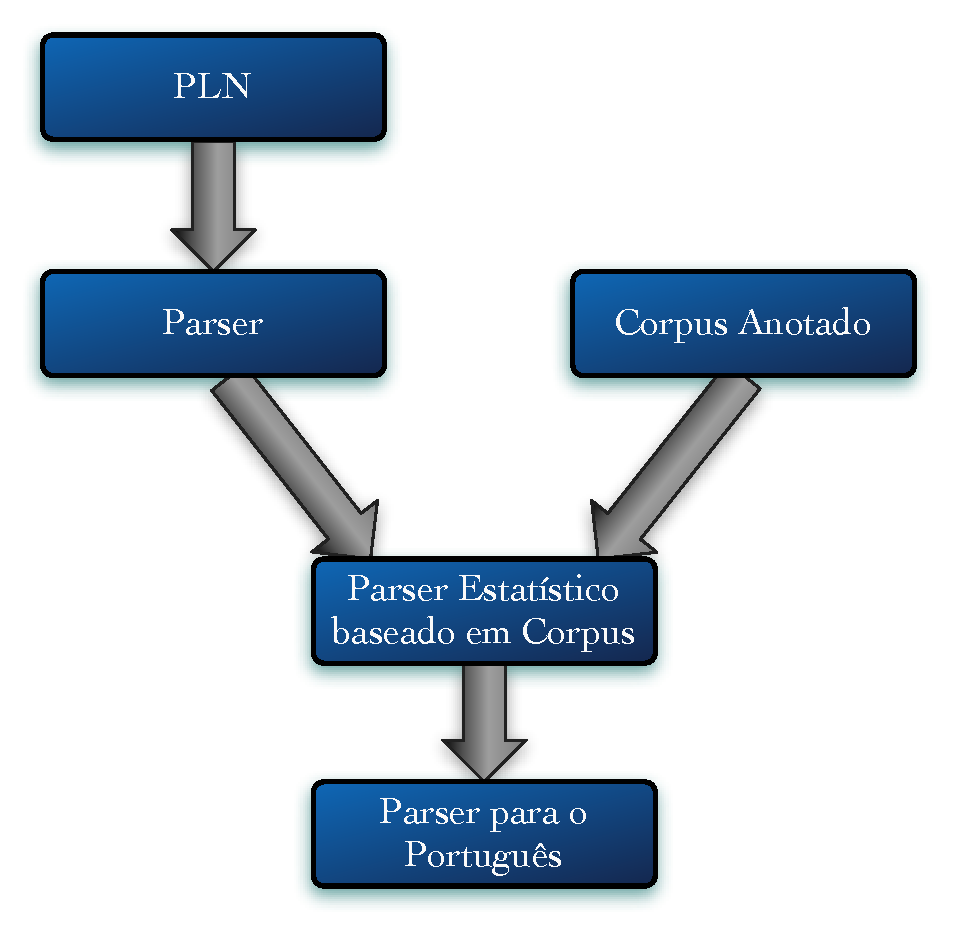
\includegraphics[scale=0.5]{fases.pdf}
		\caption{\label{fases} Insersão deste trabalho no contexto do processamento de linguagem natural propostos neste trabalho}		
	\end{center}
\end{figure}

A Figura \ref{fases} sumariza a insersão deste trabalho na área de processamento de linguagem natural. O parser desenvolvido para o português é um parser probabilístico que usa estatísticas derivadas de \emph{corpus} anotados sintaticamente para estimar os parâmetros do parser. No texto que segue abordamos alguns assuntos que fundamentam nosso trabalho.

\section{Análise de Sentença} % (fold)
\label{sec:analise_da_sentenca}

O processo de análise de sentença em linguagem natural é geralmente apresentado na literatura subdividido em vários níveis:

\begin{itemize}
	\item Análise morfológica
	\item Análise sintática
	\item Análise semântica
	\item Análise pragmática
\end{itemize}

Este trabalho foca os dois primeiros níveis de análise acima citados. Uma abordagem mais completa de todos os níveis pode ser vista em \cite{allen95,vera01} entre outros.


\subsection{Análise morfológica ou \emph{Part-of-Speech Tagging}} % (fold)
\label{sub:analise_morfologica_ou_part_of_speech_tagging}

O analisador morfológico identifica palavras ou expressões isoladas em uma sentença, sendo este processo auxiliado por delimitadores (pontuação e espaços em branco). As palavras identificadas são classificadas de acordo com seu tipo de uso ou, em linguagem natural, de acordo com sua categoria gramatical.

Neste contexto, uma instância de uma palavra em uma sentença gramaticalmente válida pode ser substituída por outra do mesmo tipo (exemplo: substantivos, pronomes, verbos, etc.), configurando uma sentença ainda válida. Para um mesmo tipo de palavra, existem grupos de regras que caracterizam o comportamento de um subconjunto de vocábulos da linguagem (exemplo: formação do plural de substantivos terminados em ``ão'', flexões dos verbos regulares terminados em ``ar'', etc.). Assim, a morfologia trata as palavras quanto à sua estrutura, forma, flexão e classificação, no que se refere a cada um dos tipos de palavras.

Esta fase é frequentemente chamada de \emph{part-of-speech tagging}, pois seu principal resultado é a determinação da categoria sintática das palavras individuais como ocorrem na sentença, também conhecida como \emph{part-of-speech} (POS). Entre essas categorias estão tipicamente as de nome (ou substantivo), verbo, preposição, etc. Outras características importantes podem ser obtidas nesta fase, como gênero (masculino ou feminino), número (singular ou plural), etc. Estas características secundárias, chamadas \emph{features} ou traços, de certa forma estendem a POS. Cada POS tem um conjunto diferenciado de \emph{features} apropriado que depende da aplicação do analisador e das concepções teóricas de quem a define. Na medida em que uma palavra é caracterizada pela sua categoria principal mais traços secundários, não é surpresa que haja uma razoável variabilidade na separação entre que características já devem estar embutidas na POS, e quais devem ser relegadas a \emph{features}. Por exemplo, algumas propostas podem selecionar como POS nome e como \emph{feature} número (singular ou plural). Outras podem atribuir POS \emph{tags} (marcações de POS) separados para nome-singular e nome-plural.

Os algoritmos para etiquetagem fundamentam-se em dois modelos mais conhecidos: os baseados em regras e os estocásticos. Os algoritmos baseados em regras, como o nome diz, fazem uso de bases de regras para identificar a categoria de um certo item lexical. Neste caso, novas regras vão sendo integradas à base à medida que novas situações de uso do item vão sendo encontradas. Os algoritmos baseados em métodos estocásticos costumam resolver as ambiguidades através de um \emph{corpus} de treino, marcado corretamente (muitas vezes através de esforço manual), calculando a probabilidade que uma certa palavra ou item lexical terá de receber uma certa etiqueta em certo contexto. O etiquetador de Eric Brill \cite{brill95}, bastante conhecido na literatura, faz uso de uma combinação desses modelos.

A escolha de um bom \emph{tagset} é fundamental para o sucesso de um \emph{parser}, embora não seja absolutamente claro como fazer este julgamento. Existem vários livros inteiros dedicados a este assunto \cite{abeille03} \cite{sardinha04}. Em linhas gerais, um bom \emph{tagset} para um \emph{parser} é aquele que possui uma boa caraterística de ""equivalência distribucional" em termos sintáticos; isto é, palavras que ocorrem tipicamente nas mesmas posições nas sentenças têm mesmo POS, enquanto que as que têm características de distribuição diferentes na mesma sentença têm POS diferente. Na abordagem de Collins \cite{collins99} que usamos neste trabalho a etiquetagem é parte integrande no algorítmo de \emph{parser}.

O conjunto de tags (\emph{tagset}) utilizado nesse trabalho é definido em \cite{florestasintatica}

\subsection{Análise sintática ou \emph{Parsing}} % (fold)
\label{sub:analise_sintatica_ou_parsing}

Através da gramática da linguagem a ser analisada e das informações do analisador morfológico, o analisador sintático procura construir árvores de derivação para cada sentença, mostrando como as palavras estão relacionadas entre si.

Durante a construção da árvore de derivação, é verificada a adequação das seqüências de palavras às regras de construção impostas pela linguagem, no processo de composição das sentenças. Dentre estas regras, pode-se citar a concordância e a regência nominal e/ou verbal, bem como o posicionamento de termos na frase.

A tarefa de um \emph{parser} para a linguagem natural é construir a estrutura sintática da sentença, dividindo-a em subconstituintes de uma forma que reflita, segundo alguma teoria da linguagem, a estrutura composicional de análise da sentença. Esta estrutura é geralmente dada como uma árvore de constituintes, em que os nodos folhas são as POS, com as respectivas palavras, e os nodos internos os conhecidos como sintagmas ou categorias sintáticas de mais alto nível.

\begin{figure}
	\begin{center}
		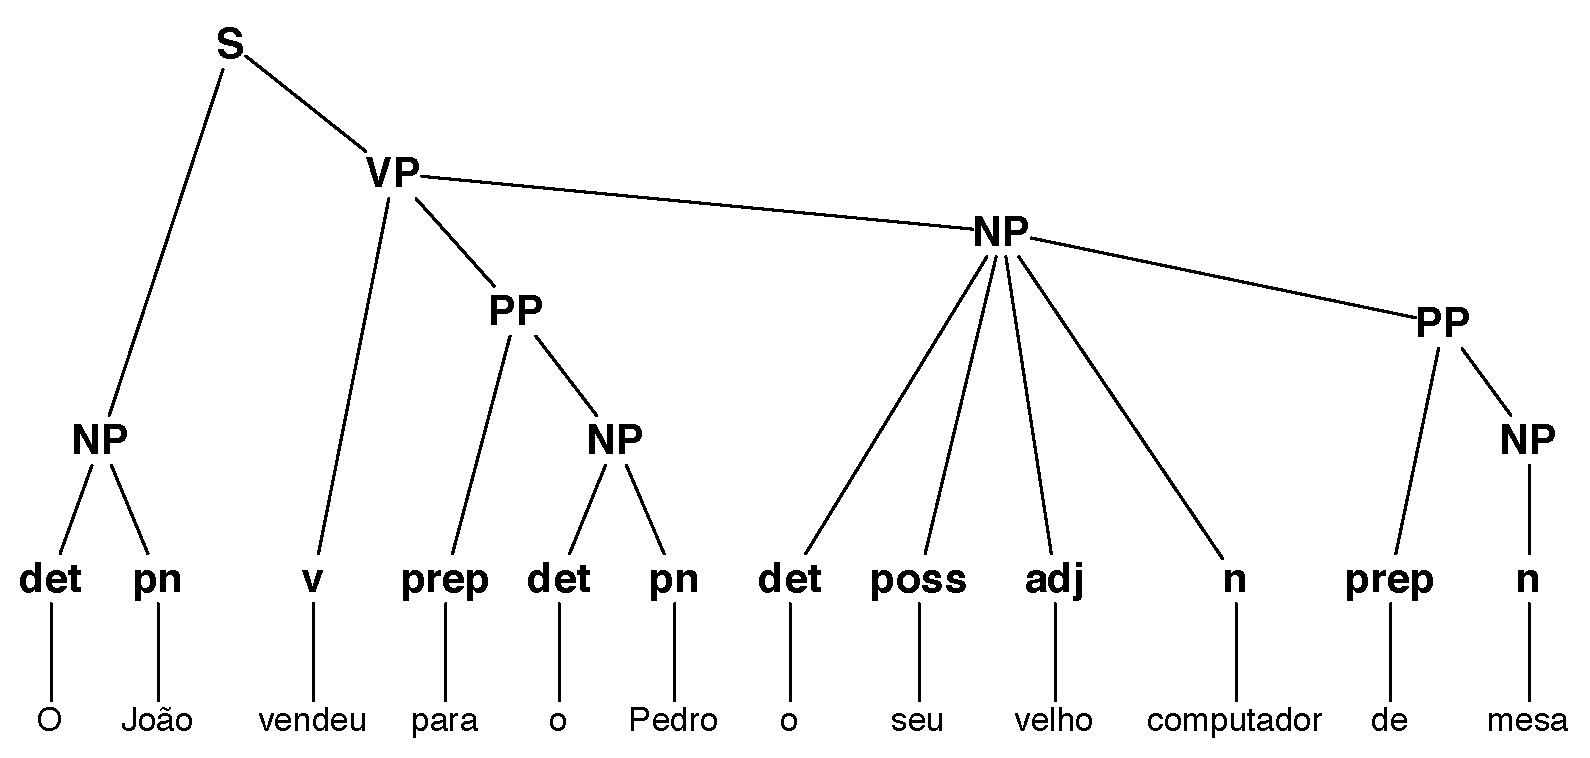
\includegraphics[scale=0.5]{tree.pdf}
		\caption{\label{tree} Árvore gramatical da frase \emph{O João vendeu para Pedro o seu velho computador de mesa}}

	\end{center}
\end{figure}

Por exemplo, a frase "O João vendeu para Pedro o seu velho computador de mesa", seria anotada gramaticalmente da seguinte forma:

\begin{verbatim}
  (S
     (NP (DET O) (PN João))
     (VP
        (V vendeu)
        (PP (PREP para) (NP (DET o) (PN Pedro)))
        (NP
            (DET o)
            (POSS seu)
            (SDJ velho)
            (N computador)
            (PP (PREP de) (NP (N mesa))))))
\end{verbatim}

			
A Figura \ref{tree} ilustra a mesma árvore em formato gráfico.

O conjunto de rótulos sintáticos utilizados nas árvores sintáticas do parser que construímos para o português esta em \cite{florestasintatica}.


% subsection análise_sintática_ou_parsing (end)

% section análise_da_sentença (end)

\section{\emph{Corpus} Anotado} % (fold)
\label{sec:corpus_anotado}

Segundo \cite{sardinha04}, \emph{corpus} é um conjunto de dados linguísticos (pertencentes ao uso oral ou escrito da língua, ou a ambos), sistematizado segundo alguns critérios, suficientemente extenso em amplitude e profundidade, de maneira que seja representativo da totalidade do uso linguístico ou de algum de seus âmbitos, disposto de tal modo que possa ser processado por computador, com a finalidade de propiciar vários, e úteis, resultados para a descrição e análise.

\emph{Corpora} anotados sintaticamente, também conhecidos como \emph{treebanks} \cite{abeille03}, são - simplificadamente - bancos de dados de sentenças anotadas com informações sintáticas e semânticas que servem como fonte de aprendizado para os sistemas estatísticos. A qualidade e o tamanho do \emph{treebank} influenciam diretamente a qualidade do resultado obtido pelo \emph{parser}. A criação do primeiro \emph{corpus} anotado data do início dos anos 60, e foi desenvolvido inicialmente para o inglês. O objetivo era prover um esquema de anotação mais completo possível, para ser utilizado por esses métodos empíricos, isto tendo em vista processamento dos corpora linguísticos. Para outras finalidades há coisas bem mais antigas

\subsection{Extensão do \emph{Corpus}} % (fold)
\label{sub:extensao_do_corpus}

A extensão e diversidade dos \emph{corpora} são definitivas na qualidade do aprendizado dos \emph{parsers} estatísticos. Conforme \cite{sardinha04}, pode-se definir três abordagens para a constituição de um \emph{corpus}.

\begin{enumerate}
\item Impressionista: baseia-se em constatações derivadas da prática da criação e da exploração de \emph{corpora}, em geral feitas por autoridades da área. Por exemplo, Aston \cite{aston97} menciona patamares que caracterizariam um \emph{corpus} pequeno (20 a 200 mil palavras) e um grande (100 milhões ou mais).

Leech \cite{leech91} fala de 1 milhão de palavras com uma taxa usual (\emph{going rate}), sugerindo o patamar mínimo. Outros são mais vagos, como Sinclair \cite{sinclair97}, que postula que o \emph{corpus} deva ser tão grande quanto a tecnologia permitir para a época, deixando subentender que a extensão de um \emph{corpus} deva variar de acordo com o padrão corrente nos grandes centros de pesquisa, que possuem equipamentos de última geração.

\item Histórica: fundamenta-se na monitoração dos \emph{corpora} eletivamente usados pela comunidade. Por exemplo, Berber Sardinha \cite{sardinha04} sugere uma classificação baseada na observação dos \emph{corpora} utilizados, segundo 4 anos de conferências de \emph{corpus}. Tabela de tamanho de \emph{corporas}:
\\




\begin{table}
   \centering
   \small
%%   \setlength{\arrayrulewidth}{2\arrayrulewidth}
%%   \setlength{\belowcaptionskip}{10pt}
   \caption{\it Tamanho de um Corpus.}

   \begin{tabular}{| c | c |}
      \hline
        \textbf{Tamanho} & \textbf{Classificação}\\
        \hline
        \hline
        Menos de 80 mil & Pequeno\\
        \hline
        80 mil a 250 mil & Pequeno-médio\\
        \hline
        250 mil a 1 milhão & Médio\\
        \hline
        1 milhão a 10 milhões & Médio-grande\\
        \hline
        10 milhões ou mais & Grande\\
        \hline

   \end{tabular}

\end{table}





\item Estatística: fundamenta-se na utilização de teorias estatísticas. Por exemplo, Biber \cite{biber93} emprega fórmulas matemáticas para identificar quantidades mínimas de palavras, gêneros e textos que se constituíram em uma amostra representativa. Algumas questões que norteiam essa abordagem são:

\begin{enumerate}
\item Dado um \emph{corpus} preexistente que serve como amostra maior, qual o tamanho mínimo de uma amostra que mantém estáveis as características da amostra maior? Essa é uma perspectiva seguida por Biber \cite{biber90,biber93}.

\item Dada uma fonte externa de referência cuja dimensão é conhecida, qual o tamanho do \emph{corpus} necessário para representar majoritariamente esta fonte? Essa vertente tem sido discutida pela comunidade de linguistas do \emph{corpus}.

\item Quanto seria perdido se o \emph{corpus} fosse de um tamanho x? Dados os recursos existentes, quais parâmetros utilizar para avalizar a decisão relativa ao tamanho de \emph{corpus} que pode ser compilado? Uma proposta segundo essa perspectiva ainda não foi formalizada, mas está presente, por exemplo, em \cite{cantossanches97.2,cantossanchez97}, que estima matematicamente a quantidade do vocabulário presente em \emph{corpora} de diversos tamanhos hipotéticos.
\end{enumerate}

\end{enumerate}

\newpage

\subsection{Corpus para processamento de linguagem natural} % (fold)
\label{sub:corpus_pln}


%%\include{vol_corpus_ingles}
\subsubsection{Corpora da Língua Inglesa}
\label{sub:corpus_ingles}

A tabela \ref{tbl:corpora} lista alguns dos corpora anotados sintaticamente mais relevantes, que são da língua inglesa.

\begin{table}
   \centering
   \small
   %%\setlength{\arrayrulewidth}{2\arrayrulewidth}
   %%\setlength{\belowcaptionskip}{10pt}
   \caption{\it Corpora da Língua Inglesa.}

   \begin{tabular}{ | p{5cm} | p{3cm} | p{3cm} | p{3cm} | }
      \hline
        \textbf{Corpus} & \textbf{Lançamento, referência na literatura} & \textbf{Palavras}& \textbf{Composição}\\
        \hline
        \hline
        Bank of English & 1987 \footnotemark[1] & 459 milhões & inglês britânico\\
        \hline
        Longman Writen American Corpus & 1997 & 100 milhões  & inglês americano, escrito ( jornais e livros )\\
        \hline
        DNC ( British National Corpus ) & 1995 & 100 milhões  & inglês britânico escrito e falado.\\
        \hline
        LLEC ( Longman-Lancaster English Language Corpus ) & 1988 & 30 milhões  & inglês de vários tipos , escrito e falado.\\
        \hline
        CHILDES (Child Language Data Exchange) & 1990 & 20 milhões & inglês infantil, falado.\\
        \hline
        The Penn TreeBank & 1989 & 10 milhões & inglês americano, escrito e falado.\\
        \hline
        Brown Corpus ( Brown University Standart Corpus of Present-day American English ) & 1964 & 1 milhão  & ingles americano, escrito\\
        \hline
   \end{tabular}
   \footnotemark[1]{Data refere-se ao Birmingham Corpus, do qual o Bank of English derivou}
   \label{tbl:corpora}
\end{table}

Existem outros corpora além dos acima elencados, que possuem um número menor de palavras. Três corpora da lista servem como marcos de referência históricos:

Brown, BNC e Bank of English. O \emph{corpus} Brown é um marco por razões óbvias: é o primeiro. O BNC é de destaque porque foi o primeiro a conter 100 milhões de palavras. Enquanto o Brown e o BNC são \emph{corpus} de amostragem, planejados e fechados, O Bank of English é um \emph{corpus} monitor, orgânico e em crescente expansão.


\subsubsection{Penn TreeBank}
\label{sub:corpus_ingles_esquema_pen}

O Penn TreeBank é um dos principais \emph{corpus} disponíveis, contem aproximadamente 7 milhões de palavras com anotação de POS, 3 milhões de palavras com ``esqueleto de parsing", mais de 2 milhões de palavras de texto anotado com informação predicado-argumento (\emph{predicate-argument structure}), e 1.6 milhões de palavras de transcrição de conversas. O material anotado possui diferentes origens e gêneros como manuais de computadores da IBM, anotações de enfermeiras, artigos do Wall Street Journal e transcrições de conversas telefônicas, entre outras.

A maioria das anotações do Penn Treebank consiste em anotação de POS, estrutura sintática e estrutura predicado-argumento dos textos escritos como os artigos do Wall Street Journal.

O conjunto de rótulos sintáticos e de POS (\emph{tagset}) usado no Penn Treebank, como muitos outros \emph{corpus}, foi baseado no Brown Corpus e é mostrado nas tabelas \ref{tbl:penn_treebank_pos} (Rótulos de Part-of-Speech) e \ref{tbl:penn_treebank_cats} (Rótulos de Categorias Sintáticas), contendo 36 tags de POS, 9 tags para pontuação e 17 tags para anotação sintática. Uma descrição detalhada do \emph{tagset} do Penn Treebank é encontrado no \emph{website} do projeto Penn Treebank em http://www.cis.upenn.edu/~treebank.

\begin{table}
   \centering
   \small
   %%\setlength{\arrayrulewidth}{2\arrayrulewidth}
   %%\setlength{\belowcaptionskip}{10pt}
   \caption{\it Rótulos de Part-of-Speech do Penn Treebank.}

   \begin{tabular}{| p{2cm} | p{4cm} | p{2cm} | p{4cm} |}

   \hline

		CC & Conjunção Coordenativa 	& 	PRP & Pronome Pessoal\\
    \hline
		CD & Numeral &   	PRP\$ & Pronome Possessivo\\
      \hline
		DT & Determinador     &		RB & Advérbio\\
      \hline
		EX & Pronome expletivo existencial ``there''     &		RBR & Advérbio, comparativo\\
      \hline
		FW & Palavra estrangeira     &		RBS & Advérbio, superlativo\\
      \hline
		IN & Preposição ou conjunção subordinada      &		RP & Partícula\\
      \hline
		JJ & Adjetivo      &		SYM & Símbolo\\
      \hline
		JJR & Adjetivo comparativo      &		TO & Qualquer ocorrência da palavra ``TO''\\
      \hline
		JJS & Adjetivo superlativo      &		UH & Interjeição\\
      \hline
		LS & Marcador de item em listas      &		VB & Verbo infinitivo\\
      \hline
		MD & Verbo auxiliar ou modal      &		VBD & Verbo passado\\
      \hline
		NN & Nome, singular      &		VBG & Verbo gerúndio ou particípio presente\\
      \hline
		NNS & Nome, plural      &		VBN & Verbo particípio passado\\
      \hline
		NP & Nome próprio singular      &		VBP & Verbo presente, exceto na terceira pessoa singular\\
      \hline
		NPS & Nome próprio plural      &		VBZ & Verbo presente, terceira pessoa singular\\
      \hline
		PDT & Predeterminador      &		WDT & Determinador interrogativo\\
      \hline
		POS & Terminador possessivo      &		WP & Pronome interrogativo\\
    \hline
     & & 	WP\$ & Pronome interrogativo possessivo\\
    \hline
     & & 	WRB & Adverbio interrogativo  \\
    \hline
     \# & Libra sinal & \$ & Caractere\$ \\
    \hline
     . & final & , & vírgula \\
    \hline
     : & dois pontos & ( & Abre parênteses \\
    \hline
     ) & Fecha parênteses & " & aspas dupla abre/fecha \\
     \hline
     ' & aspas simples & &  \\
    \hline

   \end{tabular}
   \label{tbl:penn_treebank_pos}
\end{table}


\begin{table}
   \centering
   \small
   %%\setlength{\arrayrulewidth}{2\arrayrulewidth}
   %%\setlength{\belowcaptionskip}{10pt}
   \caption{\it Rótulos de Categorias Sintáticas do Penn Treebank.}

   \begin{tabular}{ | p{2cm} | p{4cm} | p{2cm} | p{4cm} |}

   \hline
		ADJP & Sintagma Adjetivo 	& 	ADVP & Sintagma Adverbial\\
   \hline
		NP & Sintagma nominal 	& 	PP & Sintagma preposicional\\
   \hline
		S & Sintagma de clausula declarativa simples 	& 	SBAR & Sintagma de sentença subordinada\\
   \hline
		SBARQ & Sintagma de sentença interrogativa 	& 	SINV & Sintagma declarativo com inversão de sujeito\\
   \hline
		SQ & Sintagma de questão sim/não e subconstituintes de SBARQ excluindo elemento interrogativo 	& 	 VP & Sintagma verbal\\
   \hline
		WHADVP & Sintagma adverbial interrogativo 	& 	WHNP & Sintagma nominal interrogativo\\
   \hline
		WHPP & Sintagma preposicional interrogativo &    	X & Sintagma de constituinte desconhecido \\
	\hline

   \end{tabular}
   \label{tbl:penn_treebank_cats}
\end{table}

%%\include{vol_corpus_portugues}
\subsubsection{Corpora da Língua Portuguesa}
\label{sub:corpus_portugues}

Na língua portuguesa, há alguns corpora eletrônicos de destaque. A tabela \ref{tbl:corpora_port} apresenta um pequeno resumo dos \emph{corpus} existentes para o português.

\begin{table}
   \centering
   \small
   %%\setlength{\arrayrulewidth}{2\arrayrulewidth}
   %%\setlength{\belowcaptionskip}{10pt}
   \caption{\it Corpora da Língua Portuguesa.}

    \begin{tabular}{ | p{5cm} | p{3cm} | p{3cm} | p{3cm} | }
      \hline
        \textbf{Corpus} & \textbf{Palavras} & \textbf{Composição}& \textbf{Localização}\\
        \hline
        \hline

        Banco de Português &  233 milhões & português brasileiro, escrito e falado & PUC/SP \\

        \hline

        CETEMPublico ( Corpus de extração de Textos eletrônicos MCT), (Floresta Sintática, Bosque) & 220 milhões & jornal português, ``público'' & Projeto Linguateca \\

        \hline

        Corpus UNESP/Araraquara/ Usos do português & 200 milhões & português brasileiro, escrito & UNESP / Araraquara \\

        \hline

        CRPC( COrpus de referencia do português contemporâneo) & 152 milhões & português dos vários países lusófonos, com predominância da variedade européia & CLUL - Centro de lingüística da Universidade de Lisboa. \\

        \hline

        NILC & 35 milhões & português brasileiro escrito & NILC (USP, UFSCAR, UNESP Araraquara) \\
    \hline

   \end{tabular}
   \label{tbl:corpora_port}
\end{table}

\subsubsection{Floresta Sintática (Projeto Linguateca)}
\label{sub:sub_linguateca}

Um dos objetivos da Linguateca é melhorar significativamente as condições para o processamento do português, e prover recursos para pesquisa como os repositórios do Floresta Sintática , CETEMPublico e o CETEMFolha .

O CETEMPúblico (\emph{Corpus de Extractos de Textos Eletrônicos MCT/Público}) é um \emph{corpus} de aproximadamente 180 milhões de palavras em português de Portugal, criado por um projeto de processamento computacional do português após a assinatura de um protocolo entre o Ministério da Ciência e Tecnologia português (MCT) e o jornal O Público.

O CETENFolha (\emph{Corpus de Extractos de Textos Eletrônicos NILC/Folha de São Paulo}) é um \emph{corpus} de cerca de 24 milhões de palavras em português brasileiro, criado por um projeto de processamento computacional do português com base nos textos do jornal A Folha de São Paulo que fazem parte do \emph{corpus} NILC/São Carlos, compilado pelo Núcleo Interinstitucional de Lingüística Computacional (NILC).

A Floresta Sintática é um subconjunto dos corpora CETEM Público e CETEM Folha cujas sentanças foram analisadas (morfo)sintaticamente possuindo também indicação das funções sintáticas, explicitando hierarquicamente a informação relativa à estrutura de constituintes, enfim um \emph{treebank}. Foi construído como uma colaboração entre a Linguateca e o projeto VISL. Os textos foram inicialmente anotados (analisados) automaticamente pelo analisador sintático PALAVRAS (Bick 2000) e revistos manualmente por linguistas.

Atualmente, o \emph{corpus} da Floresta Sintá(c)tica tem 4 partes, que diferem quanto ao gênero textual, quanto ao modo (escrito vs falado) e quanto ao grau de revisão lingüística: o Bosque, totalmente revisto por lingüistas; a Selva, parcialmente revisto, a Floresta Virgem e a Amazônia, não revistos. Junto, todo esse material soma cerca de 261 mil frases (6.7 milhões de palavras) sintaticamente analisadas.

Para nosso estudos de desenvolvimento de um \emph{parser} probabilístico para a língua portuguesa e treino da ferramenta desenvolvida por Bikel , será utilizado o Bosque, parte da floresta sintática completamente revisada por linguistas.

O Bosque é composto por 9.368 frases, retiradas os primeiros 1000 extratos (aproximadamente) dos corpora CETENFolha e CETEMPúblico. Desde 2007, o Bosque vem passando por um novo processo de revisão, em que foram corrigidas algumas pequenas inconsistências e acrescentadas novas etiquetas. A versão final, disponível para consulta e download, é o Bosque 8.0.

Este é o \emph{corpus} mais correto da Floresta, e por isso o mais aconselhado para pesquisas em que não se prioriza tanto a quantidade, mas sim a precisão dos resultados.

Uma quantificação das etiquetas usadas no Bosque pode ser encontrada no anexo 4 da Bíblia Florestal \cite{florestasintatica}, e uma extensa documentação das opções lingüísticas tomadas durante o projeto.


\paragraph{Esquema de anotação}\label{par:corpus_bosque_esquema}\hspace*{1in}\\ \\

A Floresta Sintática foi o corpus utilizado para desenvolver o parser aqui descrito, e portanto as árvores geradas pelo parser seguem o esquema de anotação da Floresta.

Na Floresta, a cada palavra são associadas etiquetas (ou rótulos) principais (de função e de forma) e secundárias. Estas etiquetas aparecem como FUNÇÃO:forma, aonde forma corresponde ao conceito de POS. Em ``a menina gulosa", por exemplo, temos:


\begin{verbatim}
  >N:artd       a
  H:n           menina
  N<:adj        gulosa
\end{verbatim}

A anotação ``$>$N'' para a palavra ``a'' de função, e indica que a palavra em questão é dependente à esquerda (por isso o sinal ``$>$'') de um núcleo nominal (N). Já a forma de ``a'' é artigo definido. ``Menina'' é o núcleo do sintagma nominal, por isso a FUNÇÃO é H. Como a palavra em questão é um nome, a forma é n. Por fim, o adjetivo ``gulosa'' é um dependente (modificador) à direita do nome, e por isso recebe a etiqueta de FUNÇÃO (N$<$) e a etiqueta de forma adj.

A cada palavra também é associado o seu lema, e informações morfossintáticas (gênero, número, tempo, modo e pessoa para os verbos e, eventualmente, outras etiquetas indicativas de fenômenos como elipse, construções de foco etc.). As etiquetas de POS ou forma estão listadas na tabela \ref{tbl:floresta_sintatica_pos}. O rótulos sintáticos são listados na tabela \ref{tbl:floresta_sintatica_cats}.

Uma descrição detalhada do tagset da Floresta é encontrado no website do projeto Floresta Sintática em \url{http://linguateca.dei.uc.pt/Floresta/BibliaFlorestal/anexo1.html}. A versão atual do Bosque é 8.0, de 13 de Outubro de 2008, com 9.437 árvores revistas, correspondendo a 1962 extratos, 215.420 unidades e aproximadamente 183.619 palavras.

\begin{table}
   \centering
   \small
   %%\setlength{\arrayrulewidth}{2\arrayrulewidth}
   %%\setlength{\belowcaptionskip}{10pt}
   \caption{\it Tags de Part-of-Speech da Floresta Sintática.}

    \begin{tabular}{ | p{3cm} | p{10cm} |}
      \hline
        \textbf{Símbolo} & \textbf{Categoria}\\
        \hline
        \hline

    N&nome, substantivo\\
    \hline
    PROP&nome próprio\\
    \hline
    ADJ&Adjetivo\\
    \hline
    N-ADJ&flutuação entre substantivo e adjetivo\\
    \hline
    V-FIN&Verbo finito\\
    \hline
    V-INF&Infinitivo\\
    \hline
    V-PCP&Particípio passado\\
    \hline
    V-GER&Gerúndio\\
    \hline
    ART&Artigo\\
    \hline
    PRON-PERS&pronome pessoal\\
    \hline
    PRON-DET&pronome determinativo\\
    \hline
    PRON-INDP&pronome independente (com comportamento semelhante ao nome)\\
    \hline
    ADV&Advérbio\\
    \hline
    NUM&Numeral\\
    \hline
    PRP&Preposição\\
    \hline
    INTJ&Interjeição\\
    \hline
    CONJ-S&conjunção subordinativa\\
    \hline
    CONJ-C&conjunção coordenativa\\
\hline

   \end{tabular}
   \label{tbl:floresta_sintatica_pos}
\end{table}


\begin{table}
   \centering
   \small
   %%\setlength{\arrayrulewidth}{2\arrayrulewidth}
   %%\setlength{\belowcaptionskip}{10pt}
   \caption{\it Tags Sintáticos da Floresta Sintática}
   

    \begin{tabular}{ | p{3cm} | p{10cm} | }
      \hline
        \textbf{Símbolo} & \textbf{Categoria}\\
        \hline
        \hline

            NP&Sintagma nominal
            (H: nome or pronome)\\
            \hline

            ADJP&Sintagma adjetival
            (H: Adjetivo ou determinante)\\
            \hline

            ADVP&Sintagma adverbial
            (H: advérbio)\\
            \hline

            VP&Sintagma verbal
            (contém sempre MV e poderá exibir AUX)\\
            \hline

            PP&Sintagma preposicional
            (H: preposição)\\
            \hline

            CU&Sintagma evidenciador de relação de coordenação\\
            \hline

            SQ&Sequência de funções discursivas; sequência de elementos identificadores do falante, tema, etc. e do discurso propriamente dito\\


            \hline

            FCL& Oração finita\\

            \hline

            ICL&Oração infinitiva\\

            \hline

            ACL&Oração adverbial\\

            \hline


   \end{tabular}
   \label{tbl:floresta_sintatica_cats}
\end{table}


\subsubsection{Projeto Semantic Share}
\label{sub:sub_semantic_corpus}

Um objetivo principal do SemanticShare é o desenvolvimento para o português de corpora anotados da mais recente geração e da próxima geração \cite{semanticshare} - um \emph{PropBank} e um \emph{LogicalFormBank} -, dos quais uma parte é paralela a bancos de dados similares que estão a ser produzidos para outros idiomas, em outros projetos.

Estes \emph{corpora} são diferentes materializações de um banco único de enunciados e correspondentes representações gramaticais. Contêm informação morfológica, sintática e semântica integradas, armazenadas internamente em HPSG \cite{branco08}, que podem ser apresentadas em uma ou mais de dentre várias visões:

\begin{enumerate}
  \item Frases
  \item Segmentos lexicais
  \item Lemas
  \item Traços de flexão
  \item Etiquetas morfossintáticas Tabela \ref{tbl:semantic_share_cats}
  \item Entidades nomeadas e unidade multi-palavra
  \item Árvores de constituintes Tabela \ref{tbl:semantic_share_pos}
  \item Árvores de funções e papéis semânticos
  \item Formas lógicas
\end{enumerate}

São arquivadas num formato de representação interno que é linguisticamente bem informado, seguindo um quadro gramatical de primeira linha para a lingüística computacional (HPSG);

São apoiadas por ferramentas de desenvolvimento de corpora avançadas que asseguram uma extensão fácil das estruturas anotadas quando mais informação de mais dimensões lingüísticas possa ter de ser adicionada em extensões futuras (e.g. tempo, resolução de anáfora, etc), ou quando a cobertura da gramática seja aprofundada.

Estes objetivos estão ao alcance do projeto na medida em que tiram partido da maioria das ferramentas e recursos desenvolvidos pela equipa do SemanticShare em projetos anteriores bem sucedidos, nomeadamente o projeto TagShare, do qual o SemanticShare é uma continuação. Eles constituem uma coleção única de ferramentas de última geração para o Português -- segmentador de frases e lexemas, etiquetador morfossintático, lematizador, analisador morfológico, reconhecedor de entidades nomeadas --, juntamente com o respectivo \emph{corpus} de 1 milhão de ocorrências, anotado com precisão de acordo com as dimensões 1.-6. acima (serviços online em http://nlxgroup.di.fc.ul.pt).

Tudo isto será realizado com o apoio do consórcio DELPH-IN, uma iniciativa de nível mundial que visa dinamizar investigação de ponta em processamento lingüístico profundo através da partilha de ferramentas de desenvolvimento "open source", de recursos e de boas práticas (http://wiki.delph-in.net) entre os seus participantes convidados (vd. carta de convite em http://www.di.fc.ul.pt/~ahb/semanticshare.htm).

A sua plataforma tecnológica e a sua ferramenta de anotação sem rivais permitem avanços rápidos na concretização dos objetivos do projeto, dando assim continuidade à cooperação anterior, nomeadamente no quadro do projeto GramaXing, em que uma gramática para o processamento lingüístico profundo foi desenvolvida e está a ser mantida.

Para além disso, parte do banco lingüístico a ser desenvolvido é a componente portuguesa de bancos paralelos que estão a ser desenvolvidos para outros idiomas por outros membros do DELPH-IN, segundo requisitos similares.

Estes corpora anotados representam recursos chave para o processamento do Português, incluindo:


\begin{itemize}
  \item fornecer uma base empírica para o estudo lingüístico deste idioma e para o desenvolvimento de ferramentas elaboradas manualmente;
  \item treinar ferramentas de base estatística para o processamento superficial e profundo, incluindo parsers, etiquetadores de papéis semânticos, etc;
  \item avaliar ferramentas de processamento;
  \item  apoiar a experimentação de abordagens inovadoras em PLN multilingue, incluindo tradução automática estatística ou meta-anotação automática para a web semântica, etc...
\end{itemize}


\paragraph{Esquema de anotação}\label{sub:semantic_anotacao}\hspace*{1in}\\

O esquema de anotação do projeto Semantic Share são visões baseadas na anotação base do projeto que utiliza HPSG \cite{branco08}.

A partir desta anotação são extraídas ``visões'' no formato de árvores de constituintes. Estas árvores formam o \emph{corpus} de pesquisa utilizado neste trabalho.


A tabela \ref{tbl:semantic_share_pos} mostra os rótulos de POS e a tabela \ref{tbl:semantic_share_cats}, os rótulos sintáticos.

\begin{table}

   \centering
   \small
   %%\setlength{\arrayrulewidth}{2\arrayrulewidth}
   %%\setlength{\belowcaptionskip}{10pt}
   \caption{\it Tags de Part-of-Speech do projeto Semantic Share.}

    \begin{tabular}{ | p{3cm} | p{10cm} | }
      \hline
        \textbf{Símbolo} & \textbf{Categoria}\\
        \hline
        \hline

    A&Adjetivo\\
    \hline
    ADV&Adverbio\\
    \hline
    C&Complementador ( que)\\
    \hline
    CARD&Cardinal\\
    \hline
    CONJ&Conjunção\\
    \hline
    D&Determinador\\
    \hline
    DEM&Pronome demonstrativo\\
    \hline
    N&Nome\\
    \hline
    P&Preposição\\
    \hline
    PNT&Símbolo de pontuação\\
    \hline
    POSS&Pronome possessivo\\
    \hline
    PPA&Particípio passado\\
    \hline
    QNT& Quantificador\\
    \hline
    V& Verbo\\
    \hline


   \end{tabular}
\label{tbl:semantic_share_pos}      
\end{table}


\begin{table}

   \centering
   \small
   %%\setlength{\arrayrulewidth}{2\arrayrulewidth}
   %%\setlength{\belowcaptionskip}{10pt}
   \caption{\it Tags sintáticos do projeto Semantic Share.}

    \begin{tabular}{ | p{3cm} | p{10cm} | }
      \hline
        \textbf{Símbolo} & \textbf{Categoria}\\
        \hline
        \hline

        ADVP& Sintagma adverbial \\
        \hline
        AP& Sintagma Adjetival\\
        \hline
        CONJP&Sintagma coordenativo\\
        \hline
        CP&Sintagma Complementizador\\
        \hline
        NP&Sintagma nominal\\
        \hline
        N'&Projeção intermediária entre N e NP\\
        \hline
        pp&Sintagma preposicional\\
        \hline
        PPA'&Projeção intermediária entre PPA e PPAP\\
        \hline
        PPAP&Sintagma de oração Passiva\\
        \hline
        S&Sintagma de sentença\\
        \hline
        SNS&Sintagma de sentença sem sujeito\\
        \hline
        VP&Sintagma verbal\\
        \hline

   \end{tabular}
   \label{tbl:semantic_share_cats}

\end{table}

Nota: Alguns sintagma são com informação de extração, por exemplo ``S/NP'' significa sintágma de sentença com extração de NP (sujeito), VP/NP significa sintágma verbal com extração de NP (objeto), e assim por diante. As ocorrências desse tipo encontradas no \emph{corpus} foram essas: S/ADVP, S/AP, S/PP, SNS/ADVP, SNS/NP, VP/ADVP, VP/AP, VP/PP.

\newpage

%#####################################


\section{Diagrama geral do processo de \emph{parsing} estatístico baseado em \emph{corpus}} % (fold)
\label{sec:diagrama_geral_do_processo_de_parsing_estatistico_baseado_em_corpus}

\begin{figure}
	\begin{center}
		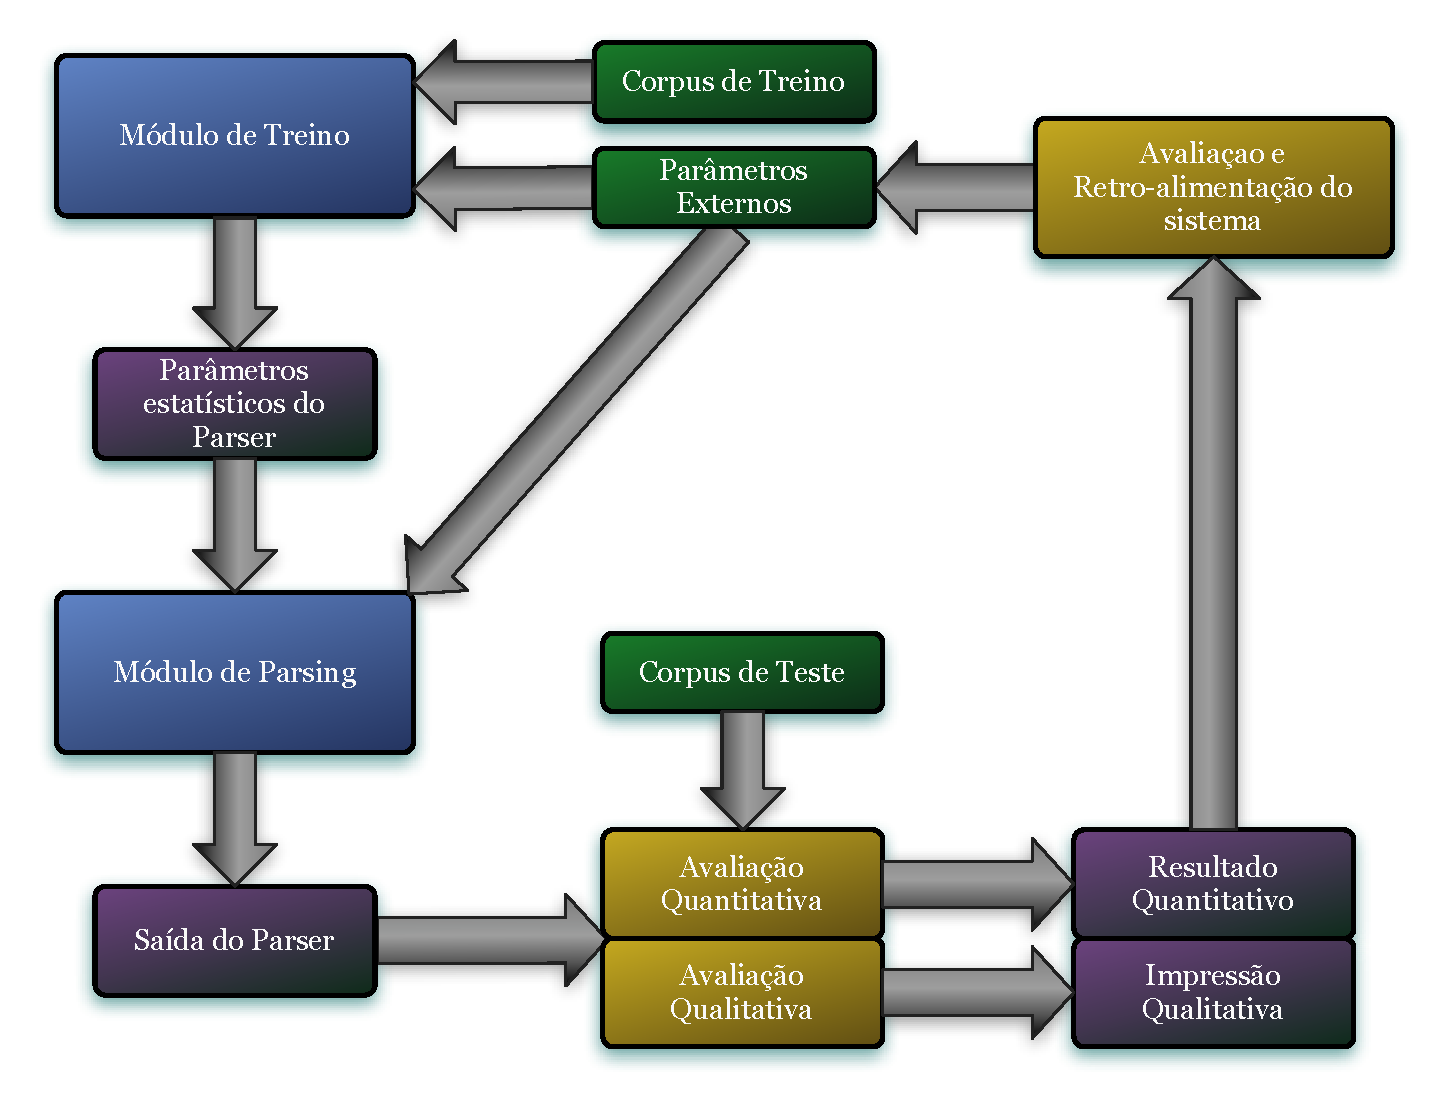
\includegraphics[scale=0.5]{parser_schema.pdf}
		\caption{\label{schema} Estágios do processamento de linguagem natural proposto pelo trabalho}		
	\end{center}
\end{figure}

Uma visão geral do processo de \emph{parsing} estatístico pode ser observada na Figura \ref{schema}.

No desenvolvimento de um \emph{parser} estatístico baseado em \emph{corpus}, o \emph{corpus} anotado é dividido em 3 partes:

\begin{enumerate}


\item{Treino: Composto por sentenças que o sistema usa para aprender.
} % (fold)
\label{sub:treino}

\item{Desenvolvimento (ou teste de desenvolvimento): 

Sentenças utilizadas para avaliar a qualidade do \emph{parser} obtidas a cada passo do desenvolvimento. Como o processo de sintonia do parser é incremental e baseado em realimentação do \emph{corpus}, pode haver uma tendência de o parser ser ajustado para se adaptar ao conjunto de sentenças submetidas aos testes. Como a análise também é qualitativa, o processo de realimentação para correção do \emph{parser} tem, fatalmente, um aspecto tendencioso. Ou seja, com o tempo, o \emph{corpus} de desenvolvimento perde a isenção para representar resultados confiáveis, pois o desenvolvedor acaba adaptando o \emph{parser} para corrigir especificamente os erros feitos naquelas sentenças. Isto é conhecido como \emph{overfitting} 
\footnote{O conceito de \emph{overfitting} é importante na aprendizagem de máquina. Geralmente, um algoritmo de aprendizagem é treinado utilizando algum conjunto de exemplos de treinamento, ou seja, situações exemplares para que a saída desejada seja acertada. Quem aprende assume como correto o que aprendeu para também ser capaz de acertar a saída correta para outros exemplos, generalizando-se a situações não apresentados durante o treinamento (baseado em seu viés indutivo). No entanto, especialmente nos casos em que a aprendizagem foi realizada muito tempo ou quando são raros exemplos de treinamento, quem aprende pode adaptar-se a muito específicas características aleatórias dos dados de treinamento, que não têm nenhuma relação causal para a função de destino. Este processo de adaptação também ocorre com relação ao conjunto de sentenças de teste e desenvolvimento se submetidos exaustivamente à análise. Neste processo de \emph{overfitting}, o desempenho nos exemplos de formação continua a aumentar, enquanto o desempenho em dados invisível torna-se pior.}. Para mitigar este efeito usa-se um terceiro conjunto de sentenças somente analisadas ao final do processo.} 

\label{sub:desenvolvimento_ou_teste_de_desenvolvimento_}




\item{Teste final: É semelhante ao de desenvolvimento, porém não é usado para sintonia do parser. O objetivo é que a avaliação sobre este \emph{corpus} seja insenta, sem efeito de \emph{overfitting}.}
\label{sub:teste_final}
\end{enumerate}


O módulo de geração do \emph{parser} tem como entrada os exemplos do \emph{corpus} de treino e gera os parâmetros estatísticos que serão utilizados pelo \emph{parser} para tomar as decisões. Este módulo é parametrizável com informações linguísticas fornecidas pelo desenvolvedor, que guiam a interpretação do \emph{corpus} de treino. Por exemplo, a informação de que, quando um constituinte tem dois nomes seguidos, o núcleo é o da esquerda para o português e é o da direita para o inglês.

O \emph{parser} gerado é composto pelo módulo de \emph{parsing} que recebe as sentenças de entrada e toma as decisões de análise guiado pelos parâmetros estatísticos aprendidos, gerando a sentença analisada.

Cada vez que uma nova versão (ou seja, um novo conjunto de parâmetros estatísticos) do \emph{parser} é gerada , ele é testado e os resultados do teste usados para realimentar o processo. Este teste é feito sobre o \emph{corpus} de desenvolvimento. Os resultados são analisados qualitativa e quantitativamente. Com base nestes valores, pode-se avaliar, por exemplo se a nova versão é melhor ou pior que as anteriores e o que se pode fazer para melhorar.


\section{\emph{Parsers} para Português} % (fold)
\label{sec:parsers_para_portugues}

Conforme mencionado anteriormente, existem alguns trabalhos de construção de \emph{parsers} para o português. Dentre eles, os de Eckhard Bick \cite{bick00}, baseado em regras, e portanto difícil de ser expandido ou adaptado; \cite{baldridge06} e \cite{bonfante03}, que também são estatísticos, baseados no modelo de Collins. Entretanto, revisando o que já referimos, os resultados até agora obtidos ainda estão distantes dos desejados.


\subsection{Trabalho de Benjamin Wing e Jason Baldridge} % (fold)
\label{sec:wing_baldridge}


Wing e Baldridge apresentaram seus resultados em \cite{baldridge06}, do desenvolvimento de um parser para o português. Assim como neste trabalho, foi utilizado como treebank o Floresta Sintática com o parser de de Dan Bikel \cite{bikel02}. Foi desenvolvido um trabalho de exploração dos diversos parâmetros possíveis na utilização do parser, e em termos de composição do treebank, foram feitas alterações nas estruturas e rótulos do treebank. 

%Uma das grandes dificuldades no trabalho de Wing e Baldridge para desenvolver um parser para o português foram com relação aos verbos, no português as inflexões verbais são significativamente mais complexas. Os verbos são conjugados em seis pessoas e em dez tempos sintéticos, além de em diversas formas não finitas. Além disso muitas terminações de verbos são idênticas aos sufixos flexionais ou derivacionais usados para formar substantivos, isso complica e muito a tarefa de análise morfológica.

Suas métricas de desempenho utilizadas foram o PARSEVAL padrão, que também utilizamos nesse trabalho, e análise de dependência não rotulada. Para a análise de dependência no entanto foi necessário um trabalho \emph{ad-hoc} de tranformação do \emph{corpus} para criação de um \emph{corpus} com as relações de dependência.

Foi provado que fazendo mudanças simples nos dados e na parametrização do parser de Bikel, incluínddo sensibilidade morfológica	do português, resulta em sensivel melhora do desempenho atingindo 63,2{\%} de PARSEVAL F-Score em sua melhor configuração. Em capítulo posterior reportaremos nossos resultados sensivelmente superiores a este.


\subsubsection{Preparando o material de treino, adaptações no \emph{corpus}} % (fold)
\label{sec:wing_baldridge_adapt_corpus}
 

Ao usar o Floresta Sintática para treino da ferramenta, Wing e Daldridge fizeram uma conversão do formato nativo para o formato PennTreebank (PTB), para este trabalho tambem tivemos que fazer tal conversão uma vez que o parser de Dan Bikel espera como entrada arquivos nesse formato. Foram feitas modificações também quando a pontuação para que esta seja melhor interpretada pelo parser em formato PTB, por exemplo '.', '?' e '!' foram marcadas como '.'. O \emph{corpus} do Floresta possui constituintes descontínuos, que na conversão foram mapeados em componentes separados.

Em principio a informação de núcleo (\emph{Head}) das sentenças geralmente marcada explicitamente no \emph{corpus} Florésta Sintática, seria de grande ajuda no processo. O PTB não contempla essa informação. Normalmente os analisadores baseados em heads das sentenças usam complexos conjuntos de heurísticas para definir os heads das sentenças durante a análise. Wing e Baldridge utilizaram-se desta marcação disponível no Floresta. No entanto, como nem todas as sentenças possuem a informação de head, Wong e Baldridge, ainda tiveram que utilizar um complexo conjunto de heurísticas para resolver as omissõese casos em que discordaram da informação constante no \emph{corpus}. Neste trabalhos optamos por ignorar a marcação fornecida no \emph{corpus} e utilizar o mecanismo disponibilizado pela ferramenta de Bikel para definir o núcleo das sentenças.

Outra mudança feita por Wing e Baldridge no \emph{corpus} foi com relação as cláusulas conjuntivas. Cláusulas conjuntivas no Floresta são normalmente marcadas com a TAG 'CU' (\emph{Coordinating conjunction})(Sintagma evidenciador de relação de coordenação), independente do tipo de constituintes coordenados. Isso faz com que no processo de treino de uma gramática, ocorram erros como confundir coordenação de sintagmas nominais com coordenações sentenciais com frequência. Foi necessário aumentar os tipos sintáticos de orações na tentativa de que essa situação não ocorresse.

Em termos de modificação das árvores do treebank outras transformações foram feitas, como aumentar cláusulas em NPs para distinguir cláusulas relativas das cláusulas em outras circunstâncias.


\subsubsection{Adaptações no analisador para o português} % (fold)
\label{sec:wing_baldridge_adapt_parser}

Foi utilizado o parser desenvolvido por Dan Bikel \cite{bikel02} para treinar e executar a análise das sentenças do português, O analisador implementa e estende os modelos de análise de Michael Collins \cite{collins99}, que inclue análise lexicalizada orientada ao núcleo das sentenças, modelos que incorporam diferentes níveis de informações estruturais, que ja foram descritas anteriormente nesse trabalho.

O modelo de análise utilizado é essencialmente o Modelo 2 de Collins \cite{collins99}.

O analisador permite extenções específicas. Além de usar o pacote em inglês para determinar uma linha de base para análise de precisão, foi criado um pacote par ao português. Este pacote fornece regras para descoberta de heads das sentenças, tratamento especial para quando os heads são explicitamente marcados, características morfológicas, e algumas opções de ajuste do analisador ao Floresta.

Modelos baseados no head das sentenças deve permitir saber quem é o filho do head anterior durante o processo de treino, Esta informação não é codificada no formato PTB, para o inglês o pacote fornece uma série de heurísticas para descobrir o head da sentença.

Para o português, para cada tipo de componente uma lista ordenada de tipos sintáticos é fornecida. modificamos essas regras como apropriado para ser utilizado com o Floresta.

Foi necessário tambem modificar o parser para indicação explícita dos heads, e utilização de arquivos de configuração dessas regras caso não esteja indicada no \emph{corpus}.

Cada pacote de idioma também pode ser codificado com base nas características morfológicas de uma palavra, estas são especificamente importantes para palavras desconhecidas. Cinco características são codificadas para cada palavra, capitalização, hifenização, numérico, inflexão e derivação. Os três primeiros indicam respectivamente se as palavras estão capitalizadas contém hífem ou estão sob forma de número. Para a maior parte, o código para crialos não precisava mudanças. Já para os dois últimos ítens tivemos que fazer modificações para trabalhar corretamente com o português. Pois como falado anteriormente, inflexões verbais e derivações no português são os grandes problemas.

As características inflexionais e derivacionais indicam a presença particular de sufixos nas palavras. Foi criado uma lista de 39 inflexões verbais ou nominais reconhecidas par ao português, isso exigiu cuidado para não bater falsos positivos e, ao mesmo tempo evitar a propagação de características das palavras. Deste modo temos únicos modos para lidar com varias terminações na terceira pessoa do plural do subjuntivo, mas separando 'ado' e 'ido' para evitar falsos positivo em substantivos como 'caldo' e 'Medo'.

Além disso algumas terminações não são listadas como 'o' e 'a', porque elas são muito ambíguas e não são exatamente nominal ou verbal. Modificações no tratamento de plural 's' também foram necessárias pois no português quase sempre o plural é indicado por uma vogal seguida de 's', mas no ingles o plural pode ocorrer com 's' depois de várias consoantes diferentes.


Outras pequenas modificações foram feitas no parser, por exemplo o modelo de Knesser-Ney foi utilizado ao invés de utilizar o padrão que é Witten-Bell. Outro exemplo foi utilizar o parametro nunkownWordThreshold=2 ao invés de 6 que é o padrão, e desligar todos os parametros que faze referencia ao PTB, e finalmente nao permitindo que oparser crie produções unárias.

 

\subsubsection{Experimentos} % (fold)
\label{sec:wing_baldridge_experimentos}

Wing e Baldridge trabalharam com três diferentes configurações de dados e parser para experimentar o parser proposto, que variam quanto ao esforço na alteração do treebank Floresta que foi utilizado como base.

A primeira configuração de testes leva em consideração o \emph{corpus} Floresta sem alteração e as configurações padrão para o inglês. A segunda configuração leva em consideração o \emph{corpus} Floresta sem alteração mas utilizando o pacote de configuração para o português. O terceiro experimento utilizou o Floresta com alterações nas suas anotações e o pacote para o português.

O primeiro representa uma abordagem mais preguiçosa, ou seja não faça nada que não seja garantir que as árvores geradas possam ser analisadas pelo parser. O segundo faz o analisador de reconhecimento da linguagem, aplicando as regras definidas para o português e as configurações ajustadas. O terceiro e último experimento envolve mudar as próprias árvores do \emph{corpus} fornecendo para o parser mais informação para o processo de análise.

Para estes experimentos foi criado um conjunto de 7497 sentenças dessas 1877 para testes e as restantes para treino.

%Foi utilizado tambem três configurações diferentes de POS tags, obtidos a partir do próprio analisador (ptags), a partir de um POS tagger externo proveniente do toolkit OpenNLP (ttags), e da Floresta em si (gtags). Este último é utilizado apenas para mostrar um limite superior sobre o desempenho do analisador para cada configuração.

O cálculo F-score para o primeiro experimento foi de 38.06{\%}, para o segundo de 63.8{\%} e para o tereceiro de 67.1{\%} 

Os desempenhos com relação a configuração básica tiveram grande melhora, simplesmente colocando definindo o pacote para português ao invés de utilizar o padrão inglês.  

Outra melhora substancial nos resultados se deve a informação de heads baseados nas regras do português informadas manualmente. Ao se adaptar um analisador como o de Bikel par auma nova linguagem vale claramente a pena colocar um mínimo de esforço para se definir um head-find rules razoavel.

\subsection{Parsing probabilístico para o português do Brasil de Andréia Gentil Bonfante} % (fold)
\label{sec:bonfante}

Bonfante em sua tese \cite{bonfante03}, faz uma investigação de métodos estatísticos quando utilizado para analisar sentenças da lingua portuguesa do Brasil. Implementando o método de modelo gerativo de Michael Collins \cite{collins99}. Como resultado apresenta uma ferramenta para processamento de linguagem natural PAPO formado por varios módulos que executam 3 funções básicas: o pré-processamento e a preparação dos dados do conjunto de sentenças usadas no treino, a geração de dois modelos probabilísticos de análise (PAPO I E PAPO II),  e um parser propriamente dito que usa um dos modelos gerados e produz as árvores sintáticas mais provaveis para uma sentença.

Nesta tese Bonfante não chegou a realizar uma avaliação abrangente e robusta de sua ferramenta, em nenhum de seus modelos. Bonfante preferiu realizar uma investigação qualitativa do desempenho do sistema, com o intuito de identificar problemas mais aparentes que surgissem na análise de um conjunto seleto de sentenças. Realizando análise apenas nas sentenças consideradas mais dificeis.

Essa avaliação inicial motivou o surgimento da versão II de sua ferramenta, que salvo um único teste, jamais teve desempenho inferior a versão inicial, na verdade superou significativamente na maioria dos casos.

Entretanto nao é possível avaliar a qualidade dos resultados tanto da versao I quanto da versão II de sua ferramenta, uma vez que Bonfante usou um volume muito pequeno de casos de teste. Foram identificados problemas quanto a ruídos na base de regras, segundo Bonfante provenientes do pré-processamento do treebank, e não originário dessa. E caracteristicas do modelo de análise sintatica do treebank utilizado que virtualmente impedem um aprendizado efetivo por parte de sua ferramenta, e que poderiam ser neutralizados de forma relativamente fácil por meio de um pré-processamento, ainda automático, mais elaborado.

Em todos os experimentos realizados na tese de Bonfante, o sistema utiliza como fonte de exemplos de análise, o CENTENFolha, proveniente do Floresta Sintática. Um \emph{corpus} de cunho jornalístico anotado com o parser simbólico e o esquema de anotação propostos e descritos por Eckhard Bick \cite{bick00}. Como este esquema de anotação tem características bastante peculiares que tornam o pré-processamento não trivial, a ponto de inclusive ser uma fonte significativa de ruído existente na entrada do gerador de modelos para sua ferramenta.

Bonfante teve que gerar um módulo de pré-processamento para as sentenças originais, um módulo de filtro de regras, que tem como entrada as sentenças do CENTENFolha e tem como saida regras, para que possam ser usadas na geração dos modelos de sua tese.

Além do filtro de regras foi preciso criar o filtro de núcleos de sentenças, os núcleos são identificados para cada regra. Para preencher o núcleo de um sintagma é necessário que seja recuperada a regra na qual ela é pai.


\subsubsection{Experimentos} % (fold)
\label{sec:bonfante_experimentos}


Para avaliara quantitativamente sua ferramenta Bonfante utilizou 23 sentenças absolutamente inéditas no sentido de não terem sido observadas no treebank utilizado para treino. Antes de serem processadas pelo seu parser de acordo com seus modelos de análise, estas sentenças foram anotadas morfossintaticamente com as TAGS do treebank.

Para cada sentença configurou-se a ferramenta para que obtivesse no máximo as dez análises mais prováveis encontradas. Caso sua ferramenta não terminasse a analise de uma sentença no prazo máximo de cinco minutos, considera sem solução.

Os resultados sao apresentados de forma quantitativa e quanto ao tempo de processamento, para processar as 23 sentenças a ferramenta levou em média 47 segundos, seus melhores resultados quanto a Precision é de 79{\%} e recall 75{\%}.

Não achamos que seus resultados sejam relevantes para avaliar a performace de sua ferramenta uma vez que apenas 23 sentenças é um universo pequeno de casos para se avaliar uma ferramenta com tal proposito.

% section parsers_para_portugues (end)






\chapter{Modelos Probabilísticos de Michael Collins}
\label{cha:michael_collins}
	\section{Gramática Livre de Contexto Probabilística}
\label{sec:pcfg}

Para descrever os modelos  probabilísticos  de \emph{parsing} de Michael Collins antes precisamos entender um pouco de Gramática Livre de Contexto Probabilística (PCFG - \emph{Probabilistic context-free grammar}).

PCFGs são uma extensão das gramáticas livres de contexto, só que existe uma probabilidade associada a cada regra de substituição.

%``''

\begin{quotation}
\footnotesize
``Segundo Bonfante (\cite{bonfante03}, p. 20), o uso de técnicas estatísticas para o aprendizado de gramáticas foi inspirado no sucesso dessas técnicas para o processamento de fala. O modelo proposto em PCFG faz uma suposição de independência que considera a probabilidade de cada regra de substituição independente de todas as outras regras usadas na derivação da sentença. A ordem de derivação não afeta o modelo. As probabilidades atribuídas às regras nas PGFGs, são encaradas como a probabilidade do sintagma-pai usando tal regra, nos subelementos descritos, em comparação a todas as outras regras que expandem o mesmo sintagma.''
\end{quotation}

\begin{quotation}
\footnotesize
``Segundo Bonfante (\cite{bonfante03}, p. 21), as gramáticas probabilísticas têm muitas vantagens. Sendo elas extensões óbvias das gramáticas livres de contexto, os algoritmos usados para GLCs podem ser transportados para as PCFGs, permitindo que todas as possíveis análises possam ser encontradas num tempo de ordem $n^3$, em que n é o tamanho da sentença.''
\end{quotation}

A ambiguidade é o maior problema na análise de sentenças. Uma gramática probabilística oferece solução para este problema, escolhendo a interpretação mais provável no momento da análise.

Vamos exemplificar: na frase ``vi o homem no monte com os binóculos", supondo a gramática parcial,

\begin{enumerate}
  \item $ S \rightarrow S \  SP^1 \ |\ SV $
  \item $ SV \rightarrow SV \ SP^2  \ |\  V \ SN \ |\ V \ SN \ SP^3 $
  \item $ SN \rightarrow SN \ SP^4  | \  N \  |  \ N \ SP^5 $
  \item $ SP \rightarrow P \ SN  $
\end{enumerate}

\begin{enumerate}
    \tiny
    \item SP modifica a sentença
    \item SP modifica o predicado
    \item SP é argumento (objeto indireto) do verbo
    \item SP modifica o sintagma nominal
    \item SP é complemento nominal
\end{enumerate}

Existe grande quantidade de árvores geradas, pois seria possível relacionar \emph{os binóculos} com \emph{no monte} com vários núcleos de sintagma como argumento ou modificador.

O caso anterior é genuinamente ambíguo (ambiguidade semântica), mas há muitos casos de ambiguidade que se devem apenas à gramática em si, ou seja, leitores percebem apenas uma interpretação.

Portanto, temos um problema quanto a descobrir qual a árvore de análise correta. Como solução poderíamos deixar que as situações de ambigüidade sejam resolvidas pela análise semântica, usar regras de desambiguação manuais ou usar modelos probabilísticos para atribuir probabilidades às diferentes árvores.

Uma gramática livre de contexto probabilística (PCFG) é uma quádrupla (N, T, $S_0$, R) onde:

 \begin{itemize}

   \item N: Conjunto de símbolos não-terminais
   \item T: Conjunto de símbolos terminais
   \item $S_0$: símbolo não-terminal, designado por símbolo inicial
   \item R: Conjunto de regras da forma $ A \rightarrow \alpha [p] $, onde:

    \begin{itemize}
      \item A é um símbolo não terminal;
      \item  $\alpha$ é uma cadeia de zero ou mais símbolos terminais e não terminais;
      \item p é um número entre 0 e 1 que representa a probabilidade condicional $P(\alpha | A)$ ( ou $P(A \rightarrow \alpha | A)$  ou de forma abreviada $P(A \rightarrow \alpha)$ ) de uma ocorrência de um dado não terminal em uma derivação ser expandida pela sequência $\alpha$.
    \end{itemize}

 \end{itemize}


$p=P(\alpha |A) = $ probabilidade de um dado não terminal A ser expandido na expressão $ \alpha. $

Sendo P uma função probabilística, a somatória das probabilidades sobre o universo de eventos deve resultar 1: 

$\sum_\alpha P(A \rightarrow \alpha)=1 $

Podemos usar uma PCFG para estimar a probabilidade associada a uma dada árvore, o que vai permitir arranjar uma solução para os casos de ambiguidade. 

Considerando a hipótese assumida pelas PCFG de que a probabilidade de expansão de cada constituinte é independente do contexto em que aparece na árvore global de análise, a probabilidade associada a cada árvore é o produto das probabilidades das regras usadas na sua derivação. Nas folhas da árvore, usam-se as probabilidades POS $P(\alpha_i|w_i)$, onde  $\alpha_i$ é a palavra e $w_i$ é a POS atribuída a palavra.

A estimativa das probabilidades associadas a cada regra pode ser feita usando um \emph{corpus} anotado de sentenças.

Supondo que haja n diferentes regras para expansão de A $A \rightarrow \alpha_i $, i de 1 a n.
\\
Pode-se então estimar $P(A \rightarrow \alpha_i|A)$ como:
\\

$ P(A \rightarrow \alpha_i) = \frac{count(A \rightarrow \alpha_i)}{\sum_{j=1}^n count(A \rightarrow \alpha_j)} = \frac{count(A \rightarrow \alpha_i)}{count(A)} $, onde count($A \rightarrow \alpha_i$) é o número de vezes que uma ocorrência de A é expandida pela regra $A \rightarrow \alpha_i$ no \emph{corpus} e count(A) é o número de vezes que uma ocorrência de A é expandida.

Consegue-se deste modo associar probabilidades às regras e construir uma gramática probabilística, por exemplo:

\begin{enumerate}
  \item  $SV \rightarrow Verbo [.50]$
  \item  $SV \rightarrow Verbo SN [.45]$
  \item  $SV \rightarrow Verbo SN SN [.05]$
\end{enumerate}

% Dado que uma árvore é constituída pelo conjunto de regras que participam na sua derivação.

\section{Trabalhos Anteriores, histórico de \emph{Parsing} Probabilístico para PLN}
\label{sec:trab_anter}


\begin{quotation}
\footnotesize
``Segundo Bonfante (\cite{bonfante03}, p. 9), o aprendizado estatístico se insere num contexto cuja linha de pesquisa é chamada de empírica, uma vez que se baseia em exemplos já prontos e aprende como lidar com aqueles ainda não vistos. A linha empiricista, que entre as décadas de 60 e 80 ficou nas sombras de crenças racionalistas encabeçadas por Chomsky (1965), cujo reflexo dentro da Inteligência Artificial caracterizava-se pela criação de sistemas inteligentes com grande quantidade de conhecimento inicial codificado à mão, ressurgiu na década de 90, com a idéia de que o conhecimento pode ser induzido a partir de algumas operações básicas de associação e generalização. Assim, segundo o empiricismo, uma máquina poderia aprender a estrutura de uma linguagem apenas observando uma grande quantidade de exemplos, usando procedimentos estatísticos gerais e métodos de associação e generalização indutiva, como aprendizado indutivo de regras.''
\end{quotation}

\begin{quotation}
\footnotesize
``Segundo Bonfante (\cite{bonfante03}, p. 10), o maior obstáculo encontrado pelos sistemas automáticos de \emph{parsing} (\emph{parsers}) surge quando estes se deparam com sentenças que possuem algum tipo de ambiguidade sintática, ou seja, sentenças com duas ou mais árvores possíveis. Por exemplo, na sentença ``A menina viu o menino de binóculo", a atribuição dos \emph{TAGS} sintáticos pode mudar a interpretação que se faz da frase. Duas árvores de representação são possíveis para a mesma sentença, nas quais, de acordo com a estrutura da primeira, a menina é que estava de binóculo e observou o menino, e na segunda, a menina observou o menino que estava de binóculo conforme ilustrado na Figura \ref{ambiguidade}. Nesses casos, é necessário que o \emph{parser} opte por uma delas, e que, de preferência, seja a que se esteja buscando.

\begin{figure}
	\begin{center}
		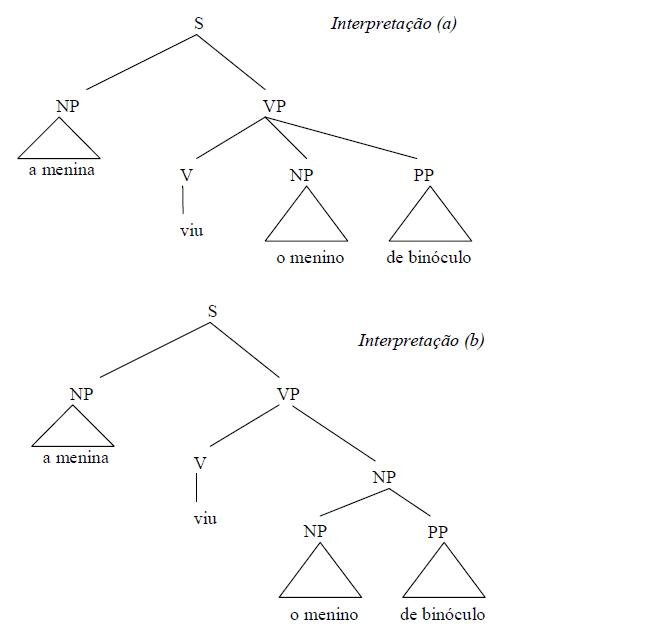
\includegraphics[scale=0.5]{ambig.jpg}
		\caption{\label{ambiguidade} Imagem das árvores da frase \emph{A menina viu o menino de binóculo}}		
	\end{center}
\end{figure}

Assim, para que o \emph{parser} pudesse fazer a atribuição procurada, ele precisaria de uma certa interpretação de significado que o ajudasse a fazer a escolha correta. No entanto, tais sistemas são totalmente desprovidos de quaisquer informações nesse sentido. Muitos acham que essa não é uma função do \emph{parser}, delegando tal responsabilidade a uma unidade especial de desambiguação. Os \emph{parsers} estatísticos utilizam medidas de probabilidades observadas em sentenças previamente analisadas como critério de desempate em prováveis ações de desambiguação. Portanto, para que funcione, é necessário que se tenha um conjunto bastante representativo de sentenças com suas respectivas árvores sintáticas. Desse modo, o \emph{parser} atribuirá probabilidades às possíveis análises de uma sentença, apresentando como resposta aquela de maior probabilidade, sendo isso feito em três passos: (1) encontra todas as possíveis análises; (2) atribui-lhes probabilidades, e (3) seleciona a de mais alta probabilidade.''
\end{quotation}

Um importante fator influenciador nas pesquisas no campo de PLN foi a disponibilização de grandes \emph{corpora} (\emph{treebanks}) anotados usados para treino dos analisadores probabilísticos.

\section{Problemas encontrados na Gramática Livre de Contexto Probabilística}
\label{sec:prob_encontrados}

Segundo Bonfante \cite{bonfante03}, PCFGs foi o ponto de início natural para as pesquisas em desenvolvimento de \emph{parsers} estatísticos para PLN. Suas propriedades formais foram bem compreendidas, algoritmos eficientes para \emph{parsing} eram bem conhecidos e descritos. Mas após algumas pesquisas descobriu-se que o uso apenas de PCFGs era insuficiente para PLN, e percepção de algumas deficiências na utilização de PCFGs em PLN gerou estudos profundos em três áreas na tentativa se achar métodos apropriados e eficientes para PLN estatística.

\begin{enumerate}
  \item Desenvolvimento de modelos mais sensíveis quanto as estruturas de linguagem.
  \item Desenvolvimento de modelos contendo parâmetros correspondentes às dependências léxicas.
  \item Desenvolvimento dos chamados ``\emph{history-based models}'' ou modelos baseados em históricos.
\end{enumerate}

\section{Métodos Probabilísticos com aumento de sensibilidade estrutural ou ao contexto}
\label{sec:aumento_sensibilidade}

Segundo Collins \cite{collins99}, muitas pesquisas foram voltadas ao objetivo de aumentar a sensibilidade ao contexto em uma PCFG, tendo resultados encorajadores. Considerando um modelo baseado em regras, mais uma vez, com mais sensibilidade ao contexto que PCFG. 

\section{Formalismo incluindo dependência lexical}
\label{sec:dependencia_lexical}

Segundo Collins \cite{collins99}, existem pelo menos duas razões para o desenvolvimento de modelos que incluem dependência de parâmetros. Primeiro, pesquisas interessadas em modelagem para reconhecimento da fala imaginavam que enquanto modelos ``\emph{trigram}'' teriam modelos sintáticos pobres, as probabilidades associadas aos pares ou triplas de palavras era muito úteis quando tinham probabilidades associadas às sentenças na linguagem. Segundo, o mais importante apontado por Michael Collins para seus estudos, pesquisas sugeriram que a dependência de probabilidade seria poderosa para abordar o problema da ambiguidade.

\section{Modelos de Michael Collins}
\label{sec:modelos_collins}

%``''

\begin{quotation}
\footnotesize
``Segundo Bonfante (\cite{bonfante03}, p. 45), Michael Collins propõe um modelo baseado em dependências lexicais entre bigramas. Este modelo usa informações lexicais para modelar relações núcleo-modificador. Também introduz um conceito de distância nesse modelo baseado em dependências entre bigramas. Segundo ele, a distância é uma variável crucial quando se decide se duas palavras estão relacionadas.

Após isso, Collins \cite{collins97} propõe três novos modelos gerativos de \emph{parsing}, que usam uma nova abordagem para melhorar o modelo de bigramas, todos eles baseados na noção \emph{head-centering}, em que o núcleo é o elemento principal e direcionador de todo o processo de geração de uma árvore sintática.

Collins define uma probabilidade conjunta P(AS; S) sobre pares árvore-sentença. Ele usa um modelo baseado no histórico de análise: uma árvore sintática é representada como uma seqüência de decisões, a partir de uma derivação \emph{top-down} e centrada no núcleo da árvore sintática. Segundo o autor, a representação da árvore sintática dessa forma permite que suposições de independência sejam feitas, levando a parâmetros condicionados a núcleos lexicais: parâmetros de projeção do núcleo, subcategorização, colocação de complemento/adjunto, dependência, distância, entre outros parâmetros.

A seguir é apresentado cada um dos modelos. O Modelo 2 representa uma evolução em relação ao Modelo 1; e o Modelo 3, em relação ao Modelo 2.''
\end{quotation}

\subsection{Modelo 1}
\label{sub:modelo1}

%``''

\begin{quotation}
\footnotesize
``Segundo Bonfante (\cite{bonfante03}, p. 53), este modelo apresenta uma proposta de como estender uma Gramática Livre de Contexto Probabilística (PCFG) para uma gramática lexicalizada (que considera itens lexicais). O Modelo 1 tem ainda parâmetros que correspondem a dependências entre pares de núcleos; a distância também é incorporada como uma medida, generalizando o modelo para uma abordagem baseada na história da análise.

A geração do lado direito da regra é quebrada em uma seqüência de pequenos passos. Cada regra passa a ter a forma:

$$Pai(nuc) = E_n(pe_n)...E_1(pe_1)NUC(nuc)D_1(pd_1)...D_m(pd_m)$$

Onde $NUC(nuc)$ representa o núcleo do sintagma, que recebe o item lexical nuc de seu pai $Pai$; $E_1...E_n e D_1...D_m$ são seus sintagmas modificadores, à esquerda e à direita de dentro do núcleo para as extremidades, com itens lexicais $pe$ e $pd$, respectivamente. As seqüências à direita e à esquerda são aumentadas com um símbolo STOP, de forma que permita um processo de Markov para o modelo. Assim, $ E_{n+1} = D_{m+1} = STOP $.

A regra de probabilidade pode ser reescrita usando a regra da cadeia de probabilidades:

$$P(E_{n+1}(pe_{n+1})...E_1(pe_1)NUC(nuc)D_1(pd_1)...D_{m+1}(pd_{m+1})|Pai(nuc)) = $$

$$P_{nuc}(NUC|Pai(nuc)) \times $$
$$\prod_{i=1..n+1} P_{esq}(E_i(pe_i)|E_1(pe_1)...E_{i-1}(pe_{i-1}), Pai(nuc),NUC) \times $$
$$\prod_{i=1..m+1} P_{dir}(D_j(pd_j)|E_1(pe_1)...E_{n+1}(pe_{n+1}),D_1(pd_1)...D_{j-1}(pd_{j-1}), Pai(nuc),NUC)  $$

Nota-se que a ordem de decomposição é: primeiro núcleo do sintagma, depois os modificadores de dentro para fora (núcleo para extremidades), sendo primeiro os modificadores a esquerda e depois os a direita.

Para um modelo ser Modelo Baseado na História da Análise ( MBHA), cada modificador poderia depender de qualquer função $\Theta$ dos modificadores anteriores, categoria do núcleo/pai e núcleo.

$$P_{esq}(E_i(pe_i)|E_1(pe_1)...E_{i-1}(pe_{i-1}), Pai(nuc),NUC) = $$
$$P_{esq}(E_i(pe_i)|\Theta(E_1(pe_1)...E_{i-1}(pe_{i-1}), Pai(nuc),NUC))$$

$$P_{dir}(D_j(pd_j)|E_1(pe_1)...E_{n+1}(pe_{n+1}),D_1(pd_1)...D_{j-1}(pd_{j-1}), Pai(nuc),NUC) = $$
$$P_{dir}(D_j(pd_j)|\Theta(E_1(pe_1)...E_{n+1}(pe_{n+1}),D_1(pd_1)...D_{j-1}(pd_{j-1}), Pai(nuc),NUC))$$

Fazendo a suposição de independência de que os modificadores são gerados independentemente uns dos outros, ou seja, fazendo $\Theta$ ignorar tudo a não ser P, NUC e nuc, temos

$$P_{esq}(E_i(pe_i)|E_1(pe_1)...E_{i-1}(pe_{i-1}), Pai(nuc),NUC) = P_{esq}(E_i(pe_i)|Pai(nuc),NUC)$$
$$P_{dir}(D_j(pd_j)|E_1(pe_1)...E_{n+1}(pe_{n+1}),D_1(pd_1)...D_{j-1}(pd_{j-1}), Pai(nuc),NUC) =$$
$$P_{dir}(D_j(pd_j)|Pai(nuc),NUC)$$

A geração de um lado direito de um regra, dado o lado esquerdo, é então feita em
três passos, sucessivamente, até que toda a árvore seja construída: (1) gera-se o núcleo (NUC); (2) geram-se modificadores à esquerda (E) e (3) geram-se modificadores à direita (D).''
\end{quotation}

\subsubsection{Adicionando Distância}
\label{sub:distancia}

\begin{quotation}
\footnotesize
``Segundo Bonfante (\cite{bonfante03}, p. 55), Michael Collins também adiciona distância a esse modelo. Essa adição é importante para capturar preferências relacionadas a modificação à direita (por exemplo, \emph{right pp attachment}) por estruturas de ligação à direita (que quase sempre traduz a preferência por dependências entre palavras adjacentes) e a preferência por dependências que não cruzam um verbo. A distância pode ser incorporada adicionando uma quantidade de dependência entre os modificadores.

$$P_{esq}(E_i(pe_i)|Pai,NUC, nuc,E_1(pe_1)...E_{i-1}(pe_{i - 1}) = $$
$$P_{esq}(E_i(pe_i)|NUC, Pai, nuc, distancia_{esq}(i - 1))$$
\\
$$P_{dir}(D_i(pd_i)|Pai,NUC, nuc,D_1(pd_1)...D_{i-1}(pd_{i - 1}) = $$
$$P_{dir}(D_i(pd_i)-NUC, Pai, nuc, distancia_{dir}(i - 1))$$
\\

A distância é um vetor contendo duas informações: adjacência (que permite aprender preferências associadas a modificadores à direita) e existência de um verbo entre eles (que permite aprender a preferência pela modificação do verbo mais recente).''
\end{quotation}

\subsection{Modelo 2}
\label{sub:modelo2}

\begin{quotation}
\footnotesize
``Segundo Bonfante (\cite{bonfante03}, p. 56), este modelo proposto por Collins, introduz a distinção entre complemento/adjunto. Os complementos  são acrescidos do sufixo ``C''. Assim, o modelo é estendido para fazer essa distinção e também para ter parâmetros que correspondam diretamente a distribuições de probabilidade sobre subcategorizações para núcleos.
O processo gerativo passa então a incluir escolha probabilística de subcategorização à esquerda ou à direita:

\begin{enumerate}
  \item Escolhe o núcleo com probabilidade $P_{nuc}(NUC|Pai, nuc)$
  \item Escolhe subcategorizações à esquerda e à direita, E-C e D-C, com probabilidades $P_{esq}(E-C|Pai,NUC, nuc)$ e $P_{dir}(D-C|Pai,NUC, nuc)$. Cada subcategorização é um conjunto que especifica os complementos que o núcleo requer como modificadores à direita ou à esquerda.
  \item Gera modificadores à esquerda e à direita com probabilidades

$P_{esq}(E_i(pe_i)|NUC, Pai, nuc, distancia_{esq}(i - 1),E - C)$ e

$P_{dir}(D_i(pd_i)|NUC, Pai, nuc, distancia_{dir}(i - 1),D - C)$

\end{enumerate}

Conforme os complementos são gerados, eles são removidos do conjunto de subcategorização (SUBCAT) apropriado. A probabilidade de gerar o símbolo STOP é 1 quando SUBCAT estiver vazio, e a probabilidade de gerar um complemento será 0 quando ela não estiver no SUBCAT.''
\end{quotation}

\subsection{Modelo 3}
\label{sub:modelo3}

\begin{quotation}
\footnotesize
``Segundo Bonfante (\cite{bonfante03}, p. 57), o modelo 3 é estendido da gramática de estrutura de frase generalizada para possibilitar tratamento de \emph{Wh-movement}\footnote{A modificação do modelo 3 não se mostra relevante e não é contemplada no \emph{parser} do Bikel, nem neste trabalho.}. Introduz parâmetros TRACES e Wh-Movement. Por exemplo, na frase ``\emph{The store that IBM bought last week}", o modelo usaria as regras para gerá-la:

\begin{enumerate}
  \item $SN \rightarrow SN SBAR(+gap)$
  \item $SBAR(+gap) \rightarrow Wh_{sn} S-C(+gap)$
  \item $S(+gap) \rightarrow SN-C SV(+gap)$
  \item $SV(+gap) \rightarrow Verbo Trace SN$
\end{enumerate}


SBAR é a representação para subcláusula; gap é a indicação de que falta algo naquele espaço.''
\end{quotation}

%\section{Casos especiais}
%\label{sec:modelo3_casos_especiais}

%Há regras especiais para derivação de coordenação e geração de símbolos de pontuação.


\chapter{Experimentos e resultados obtidos}
\label{cha:resultados_obtidos}
	\section{Metodologia}
\label{cha:metodologia}
	Este trabalho possui um forte componente experimental e exploratório. Assim, em termos metodológicos, a cada experiência realizada, os resultados obtidos foram analisados quantitativa e qualitativamente, para orientar as correções nos parâmetros do \emph{parser} ou indicar a necessidade de alterações como: a) de pré-processamento ou pós-processamento dos casos; ou b) no código do \emph{parser}. Nesse sentido, a avaliação quantitativa é um componente importante e será feita de forma rigorosa. Pretende-se utilizar os métodos de avaliação tradicionais de \emph{precision/recall} \cite{black91}.

Para trabalhar com o corpus no formato de entrada para o parser de Bikel foi necessário pré-processamento para eliminar ruídos e criar dados de entrada no formato PTB, mesmos obstáculos encontrados por Baldridge \cite{baldridge06} e Bonfante\cite{bonfante03} em seus trabalhos. 

O Corpus de treino, desenvolvimento e teste utilizado é o Bosque da Floresta Sintática que contém um total de 5200 sentenças separadas em 4160 para treino 520 para desenvolvimento e 520 para teste, nas primeiras baterias de teste utilizamos pouco menos de 100 sentenças para ajustar parâmetros mais rapidamente, na última foi utilizado 520 sentenças na fase de desenvolvimento e teste.

A presença de ruído nos dados do corpus é inevitável pois a maioria das sentenças são anotadas inicialmente de maneira automática, e mesmo após revisão manual algumas inconsistências ainda foram encontradas no decorrer do trabalho. Ruídos são possívelmente provenientes da complexidade na construções da língua que pode gerar ambiguidade ou estruturas complexas, o que dificulta a análise (em alguns casos dificulta até a análise humana). 

Não foi feita alteração quanto as TAGS utilizadas no corpus de trabalho, apenas quanto a pontuação de hífen, que será substituida por Underline.

O Conjunto de experimentos foi dividido em sub-grupos que tentam avaliar a melhor configuração com respeito a algum fator relevante ou parâmetro. Para cada grupo é eleita uma melhor configuração e a partir destes os prosseguem.

Para agilizar este processo foi desenvolvido um ambiente de testes em que os experimentos são programados e automatizados. Em particular os aspectos de pré-processamento e criação das seleções do corpus quanto a filtros necessários para diferentes experimentos.





\section{Método de Avaliação}
\label{cha:avaliacao}
	As medidas de avaliação do \emph{parser} seguirão a proposta do GEIC/Parseval \cite{black91}, adaptado conforme \cite{collins97} para ignorar pontuação e não considerar a marcação de POS na avaliação. 

Em particular, serão usadas as medidas de \emph{Labeled Precision} (LP) e \emph{Labeled Recall} (LR) e sua média harmônica ($F_{\beta=1}$) ou \emph{F-Score}, descritas abaixo:
\\
$$LP = \frac{n\acute{u}mero\; de\; constituintes\; corretos\; na\; an\acute{a}lise\; proposta}{n\acute{u}mero\; de\; constituintes\; da\; an\acute{a}lise\; proposta}$$
\\
$$LR = \frac{n\acute{u}mero\; de\; constituintes\; corretos\; na\; an\acute{a}lise\; proposta}{n\acute{u}mero\; de\; constituintes\; do\; \mathit{treebank}\; analisado}$$
\\
$$F_{\beta=1} = \frac{2*LP*LR}{LP+LR}$$
\\
O termo \emph{Labeled} se refere ao fato de que um constituinte, para contar como corretamente recuperado, deve acertar a extensão correta do texto bem como o rótulo do constituinte.

O procedimento de avaliação compara a saída do \emph{parser} com as análises anotadas no \emph{treebank}; usa a informação de parentização da representação do \emph{treebank} de uma sentença e a análise produzida pra computar três medidas: \emph{crossing brackets, precision e recall}. Neste trabalho não utilizaremos a medida de \emph{crossing brackets}.

Estas métricas são chamadas métricas estruturais, e são baseadas na avaliação dos limites dos sintagmas. Os algoritmos de \emph{parsing} têm por objetivo otimizar uma métrica em comum, que é a probabilidade de se ter uma árvore corretamente rotulada, ou seja, com uma marcação correta dos limites dos constituintes. Assim dado um nó em uma árvore sintática, a sequência de palavras dominadas por esse nó forma um sintagma, sendo o limite do sintagma representado por um intervalo inteiro \emph{[i,j]}, em que \emph{i} representa o índice da primeira palavra e \emph{j} o da última palavra do sintagma.

Black \cite{black91} propõe três medidas estruturais para avaliar sistemas de \emph{parsing}: Labeled Precision, Labeled Recall e Crossing-Brackets. Segundo Lin (1995), esse esquema de avaliação pode ser classificado como em nível de sintagma, ou nível de sentença. 
As medidas de Labeled Precision e Labeled Recall são computadas da seguinte forma:

Os limites dos sintagmas na resposta (análise produzida pelo \emph{parser}) e no \emph{gold standard} (análise do treebank) são tratados como dois conjuntos (A e K), em que A é a análise obtida do \emph{parser} proposto e K, o \emph{gold standard} do treebank a ser usado na avaliação. O Labeled Recall
é definido como a percentagem no \emph{gold standard} que também é encontrada na resposta ((A K)/K). A Labeled Precision é definida como a percentagem de limites no sintagma da resposta que também é encontrada no \emph{gold standard} ((A K)/A).

As medidas propostas no PARSEVAL partem de um pressuposto de que um constituinte está correto se corresponde ao mesmo conjunto de palavras (ignorando qualquer caractere de pontuação) e tem o mesmo rótulo que um constituinte no \emph{treebank}.

Exemplo: Considere (1) \emph{gold standard} e (2) análise do \emph{parser}:

\begin{center}
\footnotesize
\begin{verbatim}
1.  (S
      (ACL
        (NP
          (ART Um)
          (N arquitecto))
        (PP
          (PRP para)
          (NP
            (NUM 800)
            (N Km2)))))

2.  (S
      (NP
        (ART Um)
        (N arquitecto)
        (PP
          (PRP para)
          (NP
            (NUM 800)
            (N Km2)))))
\end{verbatim}
\end{center}

Temos os seguintes limites dos sintagmas:\\ \\
1. (S 0..4) (ACL 0..4) (NP 0..1) (PP 2..4) (NP 3..4)\\
2. (S 0..4) (NP 0..4) (PP 2..4) (NP 3..4)

Pontuações em (2)\footnote{No nosso caso, o S foi inserido artificialmente (não constava no treebank, mas é necessário para o formato PTB uma TAG mais externa que domine toda a sentença), não é considerado no cálculo.}: Labeled Precision = 2/3 = 66{\%}, Labeled Recall = 2/4 = 50{\%}. Essas pontuações têm que ser consideradas juntas para ter significado. 
No exemplo abaixo, teriamos 100{\%} de Labeled Precision, porém, o Labeled Recall seria apenas (2/5) = 40{\%}:

\begin{center}
\footnotesize
\begin{verbatim}
(S 
  (NP 
    (ART Um) 
    (N arquitecto)) 
  (PRP para) 
  (NUM 800) 
  (N Km2)) 
\end{verbatim}
\end{center}


\section{Resultados}
\label{cha:resultados}
	
%\begin{figure}
%	\begin{center}
%		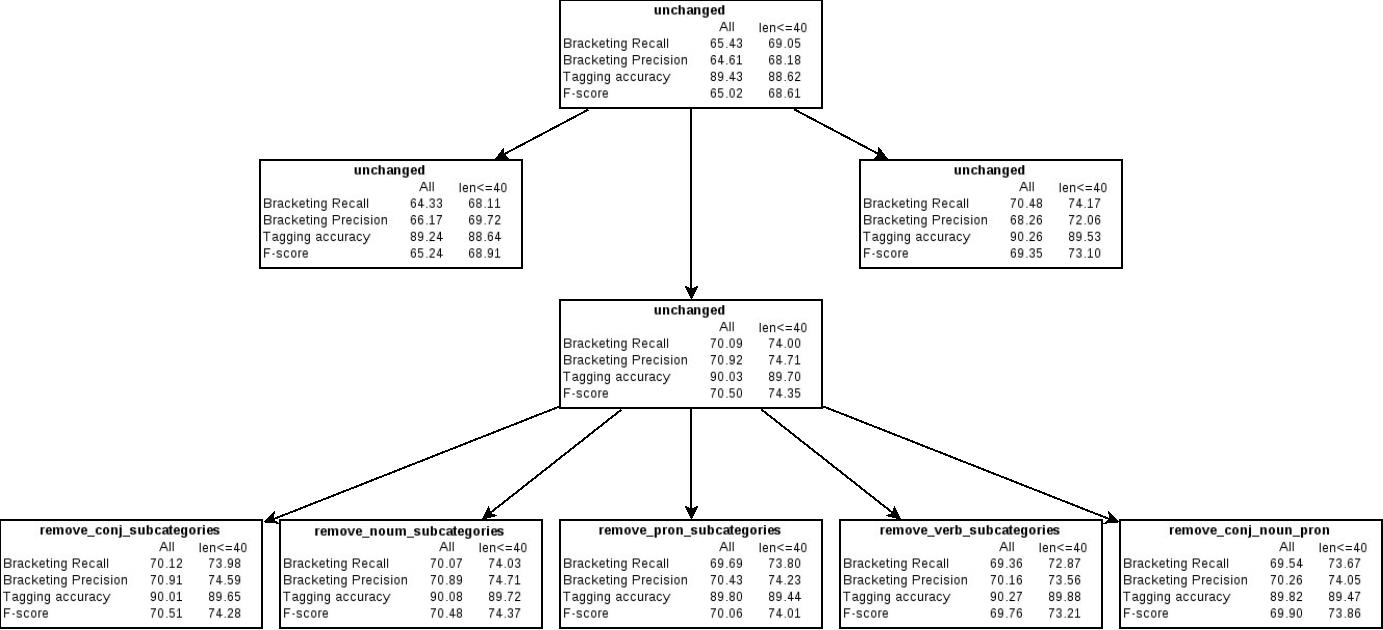
\includegraphics[scale=0.35]{diagrama_experimentos2.jpeg}
%		\caption{\label{evolucao} Evolução dos resultados }		
%	\end{center}
%\end{figure}

Primeiro teste

Regras de \emph{head-find} usadas:

\scriptsize
\begin{verbatim}
  (
  (NP (l N PROP PRON-PERS PRON-INDP N-ADJ NP))
  (VP (l V-FIN V-INF V-PCP V-GER) (l VP))
  (ADJP (l ADJ ADJP) (l PRON-DET))
  (ADVP (r ADV ADVP))
  (CU (r CONJ-C CU , ;))
  (X (l VP))
  (PP (l PRP PP))
  (FCL (l VP) (l NP))
  (ICL (l VP) (l NP))
  (ACL (l VP) (l NP))
  (* (l))
  )
\end{verbatim}

Resultados obtidos

\begin{verbatim}
  Bracketing Recall         =  62.38
  Bracketing Precision      =  68.80
  Tagging accuracy          =  58.84
\end{verbatim}

\normalsize
Achamos que os resultados estavam baixos devido as TAGS de anotação dos verbos possuírem um hífen, e o \emph{parser} não reconhece o hífen como parte da TAG.

Segundo teste

Alteramos as \emph{tags} que possuíam o caractere hífen (``-''), pois o \emph{parser} desconsidera a parte a direita do mesmo, e o programa de avaliação não. Por isso os resultados da avaliação são prejudicados.

As regras de \emph{head-find} foram alteradas para:

\scriptsize
\begin{verbatim}
  (
  (NP (l N PROP PRONPERS PRONINDP NADJ NP))
  (VP (l VFIN VINF VPCP VGER) (l VP))
  (ADJP (l ADJ ADJP) (l PRONDET))
  (ADVP (r ADV ADVP))
  (CU (r CONJC CU , ;))
  (X (l VP))
  (PP (l PRP PP))
  (FCL (l VP) (l NP))
  (ICL (l VP) (l NP))
  (ACL (l VP) (l NP))
  (* (l))
  )
\end{verbatim}

Resultados obtidos

\begin{verbatim}
  Bracketing Recall         =  61.47
  Bracketing Precision      =  68.20
  Tagging accuracy          =  79.83
\end{verbatim}

\normalsize
Apenas a precisão das tags melhorou, porém não houve melhora nas métricas \emph{Bracketing Recall} e \emph{Bracketing Precision}.

Terceiro teste

No próximo teste pretendemos verificar o quanto o \emph{parser} consegue melhorar seu desempenho quando não tem que especificar se o verbo esta em uma das quatro categorias, tendo apenas a anotação genérica de verbo.

As regras de \emph{head-find} foram alteradas para:

\scriptsize
\begin{verbatim}
  (
  (NP (l N PROP PRONPERS PRONINDP NADJ NP))
  (VP (l V) (l VP))
  (ADJP (l ADJ NUM) (l ADJP) (l PRONDET))
  (ADVP (r ADV ADVP))
  (CU (r CONJC CU , ;))
  (X (l VP))
  (PP (l PRP PP))
  (FCL (l VP) (l NP))
  (ICL (l VP) (l NP))
  (ACL (l VP) (l NP))
  (* (l))
  )
\end{verbatim}

Resultados obtidos


\begin{verbatim}
  Bracketing Recall         =  60.42
  Bracketing Precision      =  67.42
  Tagging accuracy          =  80.73
\end{verbatim}

\normalsize
Novamente, a precisão das tags aumentou, porém o \emph{Precision} e \emph{Recall} diminuíram. A generalização da tag V fez com que categorias sintáticas externas como ICL, ACL e FCL fossem influenciadas.

Quarto teste

Como já verificado com as tags, o \emph{parser} também exibe problemas com o caractere hífen (``{-}'') no texto. Após substituir todos os hífens por \emph{underscore} (``\_''), os resultados obtidos foram melhores.

As regras de \emph{head-find} são as mesmas.

\scriptsize
\begin{verbatim}
  (
  (NP (l N PROP PRONPERS PRONINDP NADJ NP))
  (VP (l V) (l VP))
  (ADJP (l ADJ NUM) (l ADJP) (l PRONDET))
  (ADVP (r ADV ADVP))
  (CU (r CONJC CU , ;))
  (X (l VP))
  (PP (l PRP PP))
  (FCL (l VP) (l NP))
  (ICL (l VP) (l NP))
  (ACL (l VP) (l NP))
  (* (l))
  )
\end{verbatim}

Resultados obtidos

\begin{verbatim}
  Bracketing Recall         =  67.42
  Bracketing Precision      =  68.09
  Tagging accuracy          =  90.36
\end{verbatim}

\normalsize

Percebemos uma melhora significativa nos valores de \emph{Bracketing Recall} e \emph{Tagging accuracy}, a partir de agora sempre substituiremos os caracteres ``{-}'' por ``\_''.

Quinto teste

Na próxima experiência vamos utilizar novamente a especialização das categorias de verbo e com um corpus de desenvolvimento e teste maior.

\scriptsize

\begin{verbatim}
  (
  (NP (l N PROP PRONPERS PRONINDP NADJ NP))
  (VP (l VFIN VINF VPCP VGER) (l VP))
  (ADJP (l ADJ ADJP) (l PRONDET))
  (ADVP (r ADV ADVP))
  (CU (r CONJC CU , ;))
  (X (l VP))
  (PP (l PRP PP))
  (FCL (l VP) (l NP))
  (ICL (l VP) (l NP))
  (ACL (l VP) (l NP))
  (* (l))
  )
\end{verbatim}


Resultados obtidos


\begin{verbatim}
  Bracketing Recall         =  72.50
  Bracketing Precision      =  72.73
  Tagging accuracy          =  90.46
\end{verbatim}

\normalsize
Verificamos uma melhora expressiva em relação aos primeiros testes realizados após a retirada dos hífens das \emph{tags} de categoria de verbos e após a substituição dos caracteres ``{-}'' por ``\_''.

Uma avaliação mais aprofundada será feita posteriormente. 




\chapter{Considerações finais e trabalhos futuros}
\label{cha:consideracoes_finais}
	
A escolha de um bom \emph{tagset} é fundamental para o sucesso de um \emph{parser}. Um bom \emph{tagset} para um \emph{parser} é aquele que possui uma boa caraterística de ``equivalência distribucional" em termos sintáticos; isto é, palavras que ocorrem tipicamente nas mesmas posições nas sentenças têm mesmo POS, enquanto que as que têm características de distribuição diferentes na mesma sentença têm POS diferente. 

Do ponto de vista experimental, obtivemos resultados de treinamento razoáveis, cuja qualidade parece bastante dependente de uma anotação bem feita. 

Um dos principais motivos de incremento nos resultados com relação a trabalhos da literatura, foi mais uma vez, com relação a construção das \emph{head-find rules} para os constituintes encontrados no corpus utilizado. O \emph{parser} de Bikel que implementa o modelo gerativo baseado na noção \emph{head-centering}, tem como principal ferramenta no processo o uso de \emph{head-find rules}, que se baseia no núcleo dos sintagmas que é o elemento principal de todo o processo de geração.

O \emph{Parser} de Bikel, além de ser possível emular os modelos de Collins, também possibilita diferentes parametrizações quanto a algoritmos utilizados e implementação de regras de \emph{head-find}, por exemplo. Alguns parâmetros melhoram a performance quanto a acertos no momento de análise de sentenças mas levam um tempo maior para finalizar, já outras configurações permitem que o tempo de análise das sentenças seja mais rápido porém a qualidade do resultado pode diminuir.

Outro fator de grande influência no incremento dos resultados foi a utilização de lematização das palavras do corpus, mais especificamente dos verbos, experimento este não abordado pelos trabalhos anteriores na literatura, acreditamos que a lematização contribuiu no processo de aprendizado do \emph{parser}.

Como trabalho futuro, sugerimos uma análise de um ponto de vista estrutural das regras implementadas por Bikel em seu \emph{parser}, pois percebemos que existem algumas regras, provavelmente de otimização, que estão \emph{hard coded} no código fonte que são dependentes do corpus utilizado originalmente (Penn TreeBank). 

Também observando a matriz de confusão apresentada nos experimentos realizados, pode-se tentar melhorar os resultados obtidos, identificando os maiores erros e possibilitando focar especificamente nesses casos. 

Também ajustes nos parâmetros que o \emph{parser} necessita para tratar as palavras desconhecidas podem levar a melhor ganho na performace.


%\chapter{Trabalhos futuros}
%\label{cha:trabsfuturos}
%	




\appendix

\chapter{Ferramenta de parsing estatístico de Dan Bikel}
\label{cha:dan_bikel1}
	Dan Bikel desenvolveu uma ferramenta de \emph{parsing} estatístico extensível que permite diferentes tipos de configuração de modelos estatísticos e gerativos, incluindo emulação dos modelos de \emph{parsing} de Michael Collins com performance semelhante. Pode ser facilmente estendida para novos domínios e novas linguagens. 

Baseada no modelo 2 de Collins \cite{collins99}, permite uma grande gama de parametrizações, implementa e estende o modelo de análise, que inclue análise lexicalizada orientada ao núcleo das sentenças, modelo que incorpora diferentes níveis de informações estruturais, que ja foram descritas anteriormente nesse trabalho. 

O analisador permite extenções específicas. Além de usar o pacote em inglês para determinar uma linha de base para análise de precisão, foi criado um pacote par ao português. Este pacote fornece regras para descoberta dos núcleos dos sintágmas, tratamento especial para quando os heads são explicitamente marcados, características morfológicas, e algumas opções de ajuste do analisador ao Floresta.

Modelos baseados no núcleo dos sintágmas deve permitir saber quem é o filho do núcleo anterior durante o processo de treino, Esta informação não é codificada no formato PTB, para o inglês o pacote fornece uma série de heurísticas para inferir o núcleo do sintágma.

A ferramenta de Dan Bikel faz uso de parâmetros que definem particularidades do seu funcionamento, sendo alterados dependendo de sua aplicação. Os parâmetros não só permitem alterar alguns comportamentos como também ``\emph{plugar}'' classes modificadas para serem usadas no lugar das classes padrões, para fazer tratamento especifico do processamento de linguagem definidos algoritmicamente.

As regras de identificação dos núcleos dos sintagmas também são configuráveis e utiliza-se para isto um arquivo de parâmetros de \emph{head-rules}, necessário para a implementação dos modelos baseados na noção \emph{head-centering}, em que o núcleo é o elemento principal e direcionador de todo o processo de geração de uma árvore sintática como falado anteriormente.

Os parâmetros estão separados em dois arquivos, arquivo de parâmetros e arquivo de regras de \emph{head-rules}, e são utilizados no momento de treinamento do \emph{parser} e no momento de analisar as frases. Os principais parâmetros são:

\section{Parâmetros de utilização do \emph{parser} de Dan Bikel}
\label{sec:bikelest_param}

\scriptsize

\textbf{O Conjunto de parâmetros abaixo permite com que o \emph{parser} de Bikel Emule o Modelo 2 definito por Michael Collins.}\\

\textbf{parser.language=english}\\
Especifica o idioma que será analisado.

\textbf{parser.language.package=danbikel.parser.english}\\
Especifica o pacote referente ao idioma analisado

\textbf{parser.language.wordFeatures=danbikel.parser.english.SimpleWordFeatures}\\
Especifica o nome da classe que estende WordFeatures no pacote da língua.

\textbf{parser.downcaseWords=false}\\
Especifica se as palavras devem ser convertidas para minúsculas durante o treino e decodificação.

\textbf{parser.subcatFactoryClass=danbikel.parser.SubcatBagFactory}\\
Especifica qual subclasse de SubcatFactory deve ser utilizada como instanciador.

\textbf{parser.shifterClass=danbikel.parser.BaseNPAwareShifter}\\
Especifica qual classe deve ser utilizada como \emph{Shifter}.

\textbf{parser.language.training=portuguese.NPArgThreadTraining}\\
Especifica qual classe que implementa a interface Training deve ser utilizada para efetuar o treinamento.

\HRule \\

\textbf{Parâmetros para classe danbikel.parser.Model}\\

\textbf{parser.model.precomputeProbabilities=true}\\
A propriedade especifica se deve ou não pré-calcular probabilidades no treino e utilização desses probabilidades pré-computada na decodificação.

\textbf{parser.model.collinsDeficientEstimation=true}\\
A propriedade especifica se deve ou não fazer estimativa deficiente de probabilidades, como o bug descrito na tese de Michael Collins.

\textbf{parser.model.prevModMapperClass=danbikel.parser.Collins}\\
Especifica qual classe que implementa a interface NonterminalMapper deve ser utilizada pelo NTMapper para mapear não-terminais que são modificadores previamente gerados de algum não-terminal \emph{head}.

\textbf{parser.model.doPruning=true}\\
A propriedade especifica se os parâmetros redundantes de cada instancia da classe Model devem ser removidos.

\textbf{parser.model.pruningThreshold=0.05}\\
A propriedade especifica um fator de quando o \emph{pruning} deve ser realizado.

\HRule \\

\textbf{Parâmetros para Modelos de Bikel, mas é ignorado quando o parâmetro danbikel.model.precomputeProbabilities é ajustado como true}\\

\textbf{parser.modelCollection.writeCanonicalEvents=true}\\
A propriedade indica ou não se a classe ModelCollection deverá salvar o (grande) \emph{HashMap} contendo as versões canônicas das instancias de \emph{Event} quando é serializado em disco. Ao decodificar usando caches ao invés de probabilidades pré-computadas (ver precomputeProbs), a criação da tabela de eventos canônicos economiza tempo, deixando o decodificador salvar no cache os eventos observados durante o treino ao invés de sempre ter que criar os eventos canônicos, dinamicamente, durante a decodificação.

\HRule \\

\textbf{Parâmetros necessários para o treinamento do parser}\\

\textbf{parser.training.addGapInfo=false}\\
Propriedade para especificar se Training.addGapInformation(Sexp) adiciona a informação de \emph{gap} ou deixa a formação da árvores intocadas.

\textbf{parser.training.collinsRelabelHeadChildrenAsArgs=true}\\
A propriedade especifica se o Training.identifyArguments(Sexp) deve re-rotular as os nodo filhos que são \emph{head} como argumentos. Essa rerotulação é desnecessária, uma vez que os \emph{heads} já são inerentemente distintos dos outros filhos, mas é realizada (e possivelmente um bug) no \emph{parser} de Collins e, por isso, está disponível como uma configuração aqui, a fim de simular o mesmo modelo.

\textbf{parser.training.collinsRepairBaseNPs=true}\\
A propriedade especifica se Training.repairBaseNPs(Sexp) altera a estrutura da árvore ou a deixa intacta.

\HRule \\

\textbf{Parâmetros para classe danbikel.parser.Trainer}\\

\textbf{parser.trainer.unknownWordThreshold=6}\\
A propriedade especifica o limite de ocorrência em que abaixo as palavras são consideradas desconhecidos pelo treinador.

\textbf{parser.trainer.countThreshold=1}\\
A propriedade especifica o limite em que abaixo as instancias de TrainerEvent são descartadas pelo treinador.

\textbf{parser.trainer.reportingInterval=1000}\\
A propriedade especifica o intervalo (em número de períodos) em que o treinador emite relatórios para System.err enquanto treina.

\textbf{parser.trainer.numPrevMods=1}\\
A propriedade especifica quantos modificadores anteriores a instancia de \emph{Trainer} deve gerar saída.

\textbf{parser.trainer.numPrevWords=1}\\
A propriedade especifica quantos núcleos (\emph{heads}) dos modificadores anteriores a instancia de \emph{Trainer} deve gerar saída.

\textbf{parser.trainer.keepAllWords=true}\\
A propriedade especifica se a instancia de \emph{Trainer} deve manter registro de todas as palavras. Normalmente, as palavras abaixo de um limite de ocorrência são mapeados como desconhecidas.

\textbf{parser.trainer.keepLowFreqTags=true}\\
A propriedade especifica se a instancia de \emph{Trainer} inclui palavras de baixa freqüência no seu mapa de POS.

\textbf{parser.trainer.collinsSkipWSJSentences=true}\\
A propriedade especifica se algumas frases são ignoradas durante o treino, a fim de emular o \emph{parser} de Michael Collins. Essa opção só deve ser utilizada com o \emph{Penn Treebank Wall Street Journal}.

\HRule \\

\textbf{Parâmetros para a classe danbikel.parser.Decoder}\\

\textbf{parser.decoder.useLowFreqTags=true}\\
A propriedade especifica se deve utilizar \emph{tags} coletadas de palavras de baixa frequência pelo treinador.

\textbf{parser.decoder.useCellLimit=false}\\
A propriedade especifica se o decodificador deve impor um limite no número de itens por célula na tabela.

\textbf{parser.decoder.cellLimit=10}\\
A propriedade especifica o limite para o número de itens que o decodificador terá por célula. Este tipo de poda só irá ocorrer se decoderUseCellLimit está ativado.

\textbf{parser.decoder.usePruneFactor=true}\\
A propriedade indica se o algoritmo deve podar ou não as arvores geradas dentro de um determinado fator.

\textbf{parser.decoder.pruneFactor=4}\\
A propriedade para especificar o fator pelo qual o decodificador deverá podar as arvores geradas. 

\textbf{parser.decoder.useCommaConstraint=true}\\
A propriedade  especifica se o decodificador deve empregar restrições sobre como vírgulas podem aparecer segundo uma regra de CFG.
$Z --> <.. X Y..>$

\textbf{parser.decoder.useHeadToParentMap=true}\\
A propriedade para especificar se o decodificador deve usar o mapeamento de nodos \emph{heads} para seus pais, derivados durante o treino.

\textbf{parser.decoder.useSimpleModNonterminalMap=true}\\
Este é mecanismo pelo qual o decodificador tenta calcular a probabilidade de um não-terminal ser modificador no contexto de um nodo pai e um núcleo.

Exemplo:\\
Se existe um NP a esquerda de um VP, cujo nodo pai é um S durante o treinamento, então o modificador não-terminal iria conter o mapeamento S, VP, left --> NP.

\textbf{Parâmetros de configuração do pacote, substitua <língua> pelo nome do pacote}\\
\textbf{parser.wordfeatures.<língua>.useUnderscores=true}\\
Propriedade que define se o símbolo ``\_'' será incluído ou não no vetor de caracteres.

\textbf{parser.headtable.<língua>=data/head-rules.lisp}\\
Define onde estão as regras de determinação dos núcleos.

\HRule \\

%\scriptsize
%\setlongtables
%\begin{longtable}{|p{3.5cm}|p{7.5cm}|p{5cm}|}
%\caption{Parâmetros do parser de Dan Bikel} \\
%\hline
%Parâmetro & Descrição & Valores válidos \\
%\hline
%\endhead
%\hline
%\endfoot
%parser.language & Especifica o idioma que será usado com a configuração & Nome do idioma, exemplo: ``portuguese'' \\
%\hline
%parser.language.package & O nome do pacote Java que será usado contendo as classes especificas para a lingua definida & Nome do pacote java, exemplo: ``parser.portuguese'' \\
%\label{tab:parâmetros}
%\end{longtable}




\section{Formato do arquivo de parâmetros}
\label{sec:bikel_formato_aqrquivo}


\scriptsize
\begin{verbatim}

#     WordNet Parser
#    Settings to emulate Mike Collins' 1997 Model 2
#
parser.language=english
parser.language.package=danbikel.parser.english
parser.language.wordFeatures=danbikel.parser.english.SimpleWordFeatures
parser.downcaseWords=false
parser.subcatFactoryClass=danbikel.parser.SubcatBagFactory
parser.shifterClass=danbikel.parser.BaseNPAwareShifter
#
# settings for danbikel.parser.Model
parser.model.precomputeProbabilities=true
parser.model.collinsDeficientEstimation=true
parser.model.prevModMapperClass=danbikel.parser.Collins
#
# settings for danbikel.parser.ModelCollection
#    the following property is ignored when
#    danbikel.model.precomputeProbabilities is true
parser.modelCollection.writeCanonicalEvents=true
#
# settings for danbikel.parser.Training
parser.training.addGapInfo=false
parser.training.collinsRelabelHeadChildrenAsArgs=true
parser.training.collinsRepairBaseNPs=true
#
# settings for danbikel.parser.Trainer
parser.trainer.unknownWordThreshold=6
parser.trainer.countThreshold=1
parser.trainer.reportingInterval=1000
parser.trainer.numPrevMods=1
parser.trainer.numPrevWords=1
parser.trainer.keepAllWords=true
parser.trainer.keepLowFreqTags=true
parser.trainer.globalModelStructureNumber=1
parser.trainer.collinsSkipWSJSentences=true
parser.trainer.modNonterminalModelStructureNumber=2
parser.trainer.modWordModelStructureNumber=2
#
# settings for danbikel.parser.CKYChart
parser.chart.itemClass=danbikel.parser.CKYItem$MappedPrevModBaseNPAware
parser.chart.collinsNPPruneHack=true
#
# settings for danbikel.parser.Decoder
parser.decoder.useLowFreqTags=true
parser.decoder.useCellLimit=false
parser.decoder.cellLimit=10
parser.decoder.usePruneFactor=true
parser.decoder.pruneFactor=4
parser.decoder.useCommaConstraint=true
parser.decoder.useHeadToParentMap=true
parser.decoder.useSimpleModNonterminalMap=true
#
#
# settings specific to language package danbikel.parser.english
#
parser.wordfeatures.english.useUnderscores=true
parser.headtable.english=data/head-rules.lisp
parser.training.metadata.english=data/training-metadata.lisp
\end{verbatim}

\normalsize

\section{Formato do arquivo de \emph{head-find rules}}
\label{sec:bikel_formato_aqrquivo_head_find}


O arquivo de \emph{head-rules} contém as regras que determinam a construção das árvores sintáticas necessárias, definindo as sentenças e seu núcleo sintático.

Abaixo segue um exemplo de definição das \emph{head-rules} utilizadas em testes de utilização do \emph{parser}.

\textbf{Regras de \emph{head-find} para anotação do Bosque}

\scriptsize

\begin{verbatim}

(
(NP (l N PROP PRONPERS PRONINDP NADJ NP))
(VP (l VFIN VINF VPCP VGER) (l VP))
(ADJP (l ADJ ADJP) (l PRONDET))
(ADVP (r ADV ADVP))
(CU (r CONJC CU , ;))
(X (l VP))
(PP (l PRP PP))
(FCL (l VP) (l NP))
(ICL (l VP) (l NP))
(ACL (l VP) (l NP))
(* (l))
)
\end{verbatim}

\normalsize

As regras definidas acima são essenciais para que no momento de treino o \emph{parser} defina exatamente a qual classe pertence as palavras classificando-as de maneira correta sintaticamente.

Por exemplo, a regra (VP (l VFIN VINF VPCP VGER) (l VP)) define que o núcleo deve ser o primeiro nodo filho, da esquerda para direita, que seja um VFIN, VINF, VPCP ou VGER. Caso não exista, então o núcleo será o mesmo do primeiro elemento, da esquerda para a direita, que seja um VP.

Serão experimentadas algumas alterações nos valores de alguns parâmetros acima citados para avaliação dos seus efeitos, e analisaremos os resultados obtidos no capitulo posterior.



\chapter{Experimentos}
\section{Head-Find Standard} % (fold)
\label{sec:exp:2009.11.19_20.59.13-remove_conj_subcategories-remove_noun_subcategories-remove_pron_subcategories-remove_verb_subcategories--headfind-standard}

Filtros Aplicados:


\begin{itemize}
  
  \item{\emph{RemoveConjSubcategories}}
  
  \item{\emph{RemoveNounSubcategories}}
  
  \item{\emph{RemovePronSubcategories}}
  
  \item{\emph{RemoveVerbSubcategories}}
  
\end{itemize}


\emph{Head-Find rules} utilizada:

\scriptsize
\begin{verbatim}
((ADJP (l NNS) (l QP) (l NN) (l $) (l ADVP) (l JJ) (l VBN) (l VBG) (l ADJP) (l JJR) (l NP) (l JJS) (l DT) (l FW) (l RBR) (l RBS) (l SBAR) (l RB))
 (ADVP (r RB) (r RBR) (r RBS) (r FW) (r ADVP) (r TO) (r CD) (r JJR) (r JJ) (r IN) (r NP) (r JJS) (r NN))
 (CONJP (r CC) (r RB) (r IN))
 (FRAG (r))
 (INTJ (l))
 (LST (r LS) (r :))
 (NAC (l NN) (l NNS) (l NNP) (l NNPS) (l NP) (l NAC) (l EX) (l $) (l CD) (l QP) (l PRP) (l VBG) (l JJ) (l JJS) (l JJR) (l ADJP) (l FW))
 (NP (r NN NNP NNPS NNS NX POS JJR)
     (l NP)
     (r $ ADJP PRN)
     (r CD)
     (r JJ JJS RB QP)
     (r))
 (PP (r IN) (r TO) (r VBG) (r VBN) (r RP) (r FW))
 (PRN (l))
 (PRT (r RP))
 (QP (l $) (l IN) (l NNS) (l NN) (l JJ) (l RB) (l DT) (l CD) (l NCD) (l QP) (l JJR) (l JJS))
 (RRC (r VP) (r NP) (r ADVP) (r ADJP) (r PP))
 (S (l TO) (l IN) (l VP) (l S) (l SBAR) (l ADJP) (l UCP) (l NP))
 (SBAR (l WHNP) (l WHPP) (l WHADVP) (l WHADJP) (l IN) (l DT) (l S) (l SQ) (l SINV) (l SBAR) (l FRAG))
 (SBARQ (l SQ) (l S) (l SINV) (l SBARQ) (l FRAG))
 (SINV (l VBZ) (l VBD) (l VBP) (l VB) (l MD) (l VP) (l S) (l SINV) (l ADJP) (l NP))
 (SQ (l VBZ) (l VBD) (l VBP) (l VB) (l MD) (l VP) (l SQ))
 (UCP (r))
 (VP (l TO) (l VBD) (l VBN) (l MD) (l VBZ) (l VB) (l VBG) (l VBP) (l VP) (l ADJP) (l NN) (l NNS) (l NP))
 (WHADJP (l CC) (l WRB) (l JJ) (l ADJP))
 (WHADVP (r CC) (r WRB))
 (WHNP (l WDT) (l WP) (l WP$) (l WHADJP) (l WHPP) (l WHNP))
 (WHPP (r IN) (r TO) (r FW))
 (* (l)))

\end{verbatim}

\normalsize

Configurações do parser:

\scriptsize
\begin{verbatim}
#     WordNet Parser
#    Settings to emulate Mike Collins' 1997 Model 2
#
parser.language=portuguese
parser.language.package=portuguese
parser.language.wordFeatures=portuguese.SimpleWordFeatures
parser.downcaseWords=false
parser.subcatFactoryClass=danbikel.parser.SubcatBagFactory
parser.shifterClass=danbikel.parser.BaseNPAwareShifter
parser.language.training=portuguese.NPArgThreadTraining
#
# settings for danbikel.parser.Model
parser.model.precomputeProbabilities=true
parser.model.collinsDeficientEstimation=true
parser.model.doPruning=true
parser.model.pruningThreshold=0.05
parser.model.prevModMapperClass=danbikel.parser.Collins
#
# settings for danbikel.parser.ModelCollection
#    the following property is ignored when
#    danbikel.model.precomputeProbabilities is true
parser.modelCollection.writeCanonicalEvents=true
#
# settings for danbikel.parser.Training
parser.training.addGapInfo=false
parser.training.collinsRelabelHeadChildrenAsArgs=false
parser.training.collinsRepairBaseNPs=false
#
# settings for danbikel.parser.Trainer
parser.trainer.unknownWordThreshold=5
parser.trainer.countThreshold=1
parser.trainer.reportingInterval=1000
parser.trainer.numPrevMods=1
parser.trainer.numPrevWords=1
parser.trainer.keepAllWords=true
parser.trainer.keepLowFreqTags=true
parser.trainer.globalModelStructureNumber=1
parser.trainer.collinsSkipWSJSentences=false
parser.trainer.modNonterminalModelStructureNumber=3
parser.trainer.modWordModelStructureNumber=2
#
# settings for danbikel.parser.CKYChart
parser.chart.itemClass=danbikel.parser.CKYItem$MappedPrevModBaseNPAware
parser.chart.collinsNPPruneHack=false
#
# settings for danbikel.parser.Decoder
parser.decoder.useLowFreqTags=true
parser.decoder.useCellLimit=false
parser.decoder.cellLimit=10
parser.decoder.usePruneFactor=true
parser.decoder.pruneFactor=3
parser.decoder.maxPruneFactor=4
parser.decoder.useCommaConstraint=true
parser.decoder.useHeadToParentMap=true
parser.decoder.useSimpleModNonterminalMap=true
#
#
# settings specific to language package portuguese
#
parser.wordfeatures.portuguese.useUnderscores=true
parser.headtable.portuguese=head-rules.lisp
parser.training.metadata.portuguese=training-metadata.lisp
\end{verbatim}

\normalsize

Resultados obtidos:

\scriptsize
\begin{verbatim}
-- All --
Number of sentence        =    522
Number of Error sentence  =      0
Number of Skip  sentence  =      0
Number of Valid sentence  =    522
Bracketing Recall         =  63.83
Bracketing Precision      =  63.98
Complete match            =   9.20
Average crossing          =   3.50
No crossing               =  34.48
2 or less crossing        =  58.05
Tagging accuracy          =  92.26

-- len<=40 --
Number of sentence        =    425
Number of Error sentence  =      0
Number of Skip  sentence  =      0
Number of Valid sentence  =    425
Bracketing Recall         =  67.99
Bracketing Precision      =  68.41
Complete match            =  11.29
Average crossing          =   2.00
No crossing               =  42.35
2 or less crossing        =  70.12
Tagging accuracy          =  92.61
No. of matched brackets   = 4481
No. of gold brackets      = 6591
No. of test brackets      = 6550
\end{verbatim}

\normalsize

% section exp:2009.11.19_20.59.13-remove_conj_subcategories-remove_noun_subcategories-remove_pron_subcategories-remove_verb_subcategories--headfind-standard (end)
\section{Head-Find Left Most} % (fold)
\label{sec:exp:2009.11.19_21.01.19-remove_conj_subcategories-remove_noun_subcategories-remove_pron_subcategories-remove_verb_subcategories--headfind-left}

Filtros Aplicados:


\begin{itemize}
  
  \item{\emph{RemoveConjSubcategories}}
  
  \item{\emph{RemoveNounSubcategories}}
  
  \item{\emph{RemovePronSubcategories}}
  
  \item{\emph{RemoveVerbSubcategories}}
  
\end{itemize}


\emph{Head-Find rules} utilizada:

\scriptsize
\begin{verbatim}
(
(* (l))
)

\end{verbatim}

\normalsize

Configurações do parser:

\scriptsize
\begin{verbatim}
#     WordNet Parser
#    Settings to emulate Mike Collins' 1997 Model 2
#
parser.language=portuguese
parser.language.package=portuguese
parser.language.wordFeatures=portuguese.SimpleWordFeatures
parser.downcaseWords=false
parser.subcatFactoryClass=danbikel.parser.SubcatBagFactory
parser.shifterClass=danbikel.parser.BaseNPAwareShifter
parser.language.training=portuguese.NPArgThreadTraining
#
# settings for danbikel.parser.Model
parser.model.precomputeProbabilities=true
parser.model.collinsDeficientEstimation=true
parser.model.doPruning=true
parser.model.pruningThreshold=0.05
parser.model.prevModMapperClass=danbikel.parser.Collins
#
# settings for danbikel.parser.ModelCollection
#    the following property is ignored when
#    danbikel.model.precomputeProbabilities is true
parser.modelCollection.writeCanonicalEvents=true
#
# settings for danbikel.parser.Training
parser.training.addGapInfo=false
parser.training.collinsRelabelHeadChildrenAsArgs=false
parser.training.collinsRepairBaseNPs=false
#
# settings for danbikel.parser.Trainer
parser.trainer.unknownWordThreshold=5
parser.trainer.countThreshold=1
parser.trainer.reportingInterval=1000
parser.trainer.numPrevMods=1
parser.trainer.numPrevWords=1
parser.trainer.keepAllWords=true
parser.trainer.keepLowFreqTags=true
parser.trainer.globalModelStructureNumber=1
parser.trainer.collinsSkipWSJSentences=false
parser.trainer.modNonterminalModelStructureNumber=3
parser.trainer.modWordModelStructureNumber=2
#
# settings for danbikel.parser.CKYChart
parser.chart.itemClass=danbikel.parser.CKYItem$MappedPrevModBaseNPAware
parser.chart.collinsNPPruneHack=false
#
# settings for danbikel.parser.Decoder
parser.decoder.useLowFreqTags=true
parser.decoder.useCellLimit=false
parser.decoder.cellLimit=10
parser.decoder.usePruneFactor=true
parser.decoder.pruneFactor=3
parser.decoder.maxPruneFactor=4
parser.decoder.useCommaConstraint=true
parser.decoder.useHeadToParentMap=true
parser.decoder.useSimpleModNonterminalMap=true
#
#
# settings specific to language package portuguese
#
parser.wordfeatures.portuguese.useUnderscores=true
parser.headtable.portuguese=head-rules.lisp
parser.training.metadata.portuguese=training-metadata.lisp
\end{verbatim}

\normalsize

Resultados obtidos:

\scriptsize
\begin{verbatim}
-- All --
Number of sentence        =    522
Number of Error sentence  =      0
Number of Skip  sentence  =      0
Number of Valid sentence  =    522
Bracketing Recall         =  68.40
Bracketing Precision      =  67.58
Complete match            =  10.15
Average crossing          =   3.02
No crossing               =  36.21
2 or less crossing        =  61.11
Tagging accuracy          =  92.87

-- len<=40 --
Number of sentence        =    425
Number of Error sentence  =      0
Number of Skip  sentence  =      0
Number of Valid sentence  =    425
Bracketing Recall         =  72.11
Bracketing Precision      =  71.51
Complete match            =  12.47
Average crossing          =   1.73
No crossing               =  44.00
2 or less crossing        =  72.94
Tagging accuracy          =  93.02
No. of matched brackets   = 4753
No. of gold brackets      = 6591
No. of test brackets      = 6647
\end{verbatim}

\normalsize

% section exp:2009.11.19_21.01.19-remove_conj_subcategories-remove_noun_subcategories-remove_pron_subcategories-remove_verb_subcategories--headfind-left (end)
\section{Head-Find Right Most} % (fold)
\label{sec:exp:2009.11.19_21.02.34-remove_conj_subcategories-remove_noun_subcategories-remove_pron_subcategories-remove_verb_subcategories--headfind-right}

Filtros Aplicados:


\begin{itemize}
  
  \item{\emph{RemoveConjSubcategories}}
  
  \item{\emph{RemoveNounSubcategories}}
  
  \item{\emph{RemovePronSubcategories}}
  
  \item{\emph{RemoveVerbSubcategories}}
  
\end{itemize}


\emph{Head-Find rules} utilizada:

\scriptsize
\begin{verbatim}
(
(* (r))
)

\end{verbatim}

\normalsize

Configurações do parser:

\scriptsize
\begin{verbatim}
#     WordNet Parser
#    Settings to emulate Mike Collins' 1997 Model 2
#
parser.language=portuguese
parser.language.package=portuguese
parser.language.wordFeatures=portuguese.SimpleWordFeatures
parser.downcaseWords=false
parser.subcatFactoryClass=danbikel.parser.SubcatBagFactory
parser.shifterClass=danbikel.parser.BaseNPAwareShifter
parser.language.training=portuguese.NPArgThreadTraining
#
# settings for danbikel.parser.Model
parser.model.precomputeProbabilities=true
parser.model.collinsDeficientEstimation=true
parser.model.doPruning=true
parser.model.pruningThreshold=0.05
parser.model.prevModMapperClass=danbikel.parser.Collins
#
# settings for danbikel.parser.ModelCollection
#    the following property is ignored when
#    danbikel.model.precomputeProbabilities is true
parser.modelCollection.writeCanonicalEvents=true
#
# settings for danbikel.parser.Training
parser.training.addGapInfo=false
parser.training.collinsRelabelHeadChildrenAsArgs=false
parser.training.collinsRepairBaseNPs=false
#
# settings for danbikel.parser.Trainer
parser.trainer.unknownWordThreshold=5
parser.trainer.countThreshold=1
parser.trainer.reportingInterval=1000
parser.trainer.numPrevMods=1
parser.trainer.numPrevWords=1
parser.trainer.keepAllWords=true
parser.trainer.keepLowFreqTags=true
parser.trainer.globalModelStructureNumber=1
parser.trainer.collinsSkipWSJSentences=false
parser.trainer.modNonterminalModelStructureNumber=3
parser.trainer.modWordModelStructureNumber=2
#
# settings for danbikel.parser.CKYChart
parser.chart.itemClass=danbikel.parser.CKYItem$MappedPrevModBaseNPAware
parser.chart.collinsNPPruneHack=false
#
# settings for danbikel.parser.Decoder
parser.decoder.useLowFreqTags=true
parser.decoder.useCellLimit=false
parser.decoder.cellLimit=10
parser.decoder.usePruneFactor=true
parser.decoder.pruneFactor=3
parser.decoder.maxPruneFactor=4
parser.decoder.useCommaConstraint=true
parser.decoder.useHeadToParentMap=true
parser.decoder.useSimpleModNonterminalMap=true
#
#
# settings specific to language package portuguese
#
parser.wordfeatures.portuguese.useUnderscores=true
parser.headtable.portuguese=head-rules.lisp
parser.training.metadata.portuguese=training-metadata.lisp
\end{verbatim}

\normalsize

Resultados obtidos:

\scriptsize
\begin{verbatim}
-- All --
Number of sentence        =    522
Number of Error sentence  =      0
Number of Skip  sentence  =      0
Number of Valid sentence  =    522
Bracketing Recall         =  64.30
Bracketing Precision      =  66.44
Complete match            =  11.30
Average crossing          =   3.22
No crossing               =  35.44
2 or less crossing        =  56.51
Tagging accuracy          =  92.09

-- len<=40 --
Number of sentence        =    425
Number of Error sentence  =      0
Number of Skip  sentence  =      0
Number of Valid sentence  =    425
Bracketing Recall         =  68.53
Bracketing Precision      =  70.44
Complete match            =  13.88
Average crossing          =   1.98
No crossing               =  43.53
2 or less crossing        =  68.24
Tagging accuracy          =  92.39
No. of matched brackets   = 4517
No. of gold brackets      = 6591
No. of test brackets      = 6413
\end{verbatim}

\normalsize

% section exp:2009.11.19_21.02.34-remove_conj_subcategories-remove_noun_subcategories-remove_pron_subcategories-remove_verb_subcategories--headfind-right (end)
\section{Head-Find Português} % (fold)
\label{sec:exp:2009.11.19_21.03.53-remove_conj_subcategories-remove_noun_subcategories-remove_pron_subcategories-remove_verb_subcategories--headfind-pt}

Filtros Aplicados:


\begin{itemize}
  
  \item{\emph{RemoveConjSubcategories}}
  
  \item{\emph{RemoveNounSubcategories}}
  
  \item{\emph{RemovePronSubcategories}}
  
  \item{\emph{RemoveVerbSubcategories}}
  
\end{itemize}


\emph{Head-Find rules} utilizada:

\scriptsize
\begin{verbatim}
(
(NP (l N PROP PRON_PERS PRON_INDP PRON NADJ NP))
(VP (l V_FIN V_INF V_PCP V_GER V) (l VP))
(ADJP (l ADJ ADJP) (l PRON_DET PRON))
(ADVP (r ADV ADVP))
(CU (r CONJ_C CONJ CU , ;))
(X (l VP))
(PP (l PRP PP))
(FCL (l VP) (l NP))
(ICL (l VP) (l NP))
(ACL (l VP) (l NP))
(* (l))
)

\end{verbatim}

\normalsize

Configurações do parser:

\scriptsize
\begin{verbatim}
#     WordNet Parser
#    Settings to emulate Mike Collins' 1997 Model 2
#
parser.language=portuguese
parser.language.package=portuguese
parser.language.wordFeatures=portuguese.SimpleWordFeatures
parser.downcaseWords=false
parser.subcatFactoryClass=danbikel.parser.SubcatBagFactory
parser.shifterClass=danbikel.parser.BaseNPAwareShifter
parser.language.training=portuguese.NPArgThreadTraining
#
# settings for danbikel.parser.Model
parser.model.precomputeProbabilities=true
parser.model.collinsDeficientEstimation=true
parser.model.doPruning=true
parser.model.pruningThreshold=0.05
parser.model.prevModMapperClass=danbikel.parser.Collins
#
# settings for danbikel.parser.ModelCollection
#    the following property is ignored when
#    danbikel.model.precomputeProbabilities is true
parser.modelCollection.writeCanonicalEvents=true
#
# settings for danbikel.parser.Training
parser.training.addGapInfo=false
parser.training.collinsRelabelHeadChildrenAsArgs=false
parser.training.collinsRepairBaseNPs=false
#
# settings for danbikel.parser.Trainer
parser.trainer.unknownWordThreshold=5
parser.trainer.countThreshold=1
parser.trainer.reportingInterval=1000
parser.trainer.numPrevMods=1
parser.trainer.numPrevWords=1
parser.trainer.keepAllWords=true
parser.trainer.keepLowFreqTags=true
parser.trainer.globalModelStructureNumber=1
parser.trainer.collinsSkipWSJSentences=false
parser.trainer.modNonterminalModelStructureNumber=3
parser.trainer.modWordModelStructureNumber=2
#
# settings for danbikel.parser.CKYChart
parser.chart.itemClass=danbikel.parser.CKYItem$MappedPrevModBaseNPAware
parser.chart.collinsNPPruneHack=false
#
# settings for danbikel.parser.Decoder
parser.decoder.useLowFreqTags=true
parser.decoder.useCellLimit=false
parser.decoder.cellLimit=10
parser.decoder.usePruneFactor=true
parser.decoder.pruneFactor=3
parser.decoder.maxPruneFactor=4
parser.decoder.useCommaConstraint=true
parser.decoder.useHeadToParentMap=true
parser.decoder.useSimpleModNonterminalMap=true
#
#
# settings specific to language package portuguese
#
parser.wordfeatures.portuguese.useUnderscores=true
parser.headtable.portuguese=head-rules.lisp
parser.training.metadata.portuguese=training-metadata.lisp
\end{verbatim}

\normalsize

Resultados obtidos:

\scriptsize
\begin{verbatim}
-- All --
Number of sentence        =    522
Number of Error sentence  =      0
Number of Skip  sentence  =      0
Number of Valid sentence  =    522
Bracketing Recall         =  68.46
Bracketing Precision      =  68.95
Complete match            =  13.60
Average crossing          =   3.00
No crossing               =  36.40
2 or less crossing        =  61.49
Tagging accuracy          =  92.78

-- len<=40 --
Number of sentence        =    425
Number of Error sentence  =      0
Number of Skip  sentence  =      0
Number of Valid sentence  =    425
Bracketing Recall         =  72.95
Bracketing Precision      =  73.62
Complete match            =  16.71
Average crossing          =   1.77
No crossing               =  44.71
2 or less crossing        =  74.35
Tagging accuracy          =  92.94
No. of matched brackets   = 4808
No. of gold brackets      = 6591
No. of test brackets      = 6531
\end{verbatim}

\normalsize

% section exp:2009.11.19_21.03.53-remove_conj_subcategories-remove_noun_subcategories-remove_pron_subcategories-remove_verb_subcategories--headfind-pt (end)
\section{Com subcategorias de V} % (fold)
\label{sec:exp:2009.11.19_21.05.31-remove_conj_subcategories-remove_noun_subcategories-remove_pron_subcategories}

Filtros Aplicados:


\begin{itemize}
  
  \item{\emph{RemoveConjSubcategories}}
  
  \item{\emph{RemoveNounSubcategories}}
  
  \item{\emph{RemovePronSubcategories}}
  
\end{itemize}


\emph{Head-Find rules} utilizada:

\scriptsize
\begin{verbatim}
(
(NP (l N PROP PRON_PERS PRON_INDP PRON NADJ NP))
(VP (l V_FIN V_INF V_PCP V_GER V) (l VP))
(ADJP (l ADJ ADJP) (l PRON_DET PRON))
(ADVP (r ADV ADVP))
(CU (r CONJ_C CONJ CU , ;))
(X (l VP))
(PP (l PRP PP))
(FCL (l VP) (l NP))
(ICL (l VP) (l NP))
(ACL (l VP) (l NP))
(* (l))
)

\end{verbatim}

\normalsize

Configurações do parser:

\scriptsize
\begin{verbatim}
#     WordNet Parser
#    Settings to emulate Mike Collins' 1997 Model 2
#
parser.language=portuguese
parser.language.package=portuguese
parser.language.wordFeatures=portuguese.SimpleWordFeatures
parser.downcaseWords=false
parser.subcatFactoryClass=danbikel.parser.SubcatBagFactory
parser.shifterClass=danbikel.parser.BaseNPAwareShifter
parser.language.training=portuguese.NPArgThreadTraining
#
# settings for danbikel.parser.Model
parser.model.precomputeProbabilities=true
parser.model.collinsDeficientEstimation=true
parser.model.doPruning=true
parser.model.pruningThreshold=0.05
parser.model.prevModMapperClass=danbikel.parser.Collins
#
# settings for danbikel.parser.ModelCollection
#    the following property is ignored when
#    danbikel.model.precomputeProbabilities is true
parser.modelCollection.writeCanonicalEvents=true
#
# settings for danbikel.parser.Training
parser.training.addGapInfo=false
parser.training.collinsRelabelHeadChildrenAsArgs=false
parser.training.collinsRepairBaseNPs=false
#
# settings for danbikel.parser.Trainer
parser.trainer.unknownWordThreshold=5
parser.trainer.countThreshold=1
parser.trainer.reportingInterval=1000
parser.trainer.numPrevMods=1
parser.trainer.numPrevWords=1
parser.trainer.keepAllWords=true
parser.trainer.keepLowFreqTags=true
parser.trainer.globalModelStructureNumber=1
parser.trainer.collinsSkipWSJSentences=false
parser.trainer.modNonterminalModelStructureNumber=3
parser.trainer.modWordModelStructureNumber=2
#
# settings for danbikel.parser.CKYChart
parser.chart.itemClass=danbikel.parser.CKYItem$MappedPrevModBaseNPAware
parser.chart.collinsNPPruneHack=false
#
# settings for danbikel.parser.Decoder
parser.decoder.useLowFreqTags=true
parser.decoder.useCellLimit=false
parser.decoder.cellLimit=10
parser.decoder.usePruneFactor=true
parser.decoder.pruneFactor=3
parser.decoder.maxPruneFactor=4
parser.decoder.useCommaConstraint=true
parser.decoder.useHeadToParentMap=true
parser.decoder.useSimpleModNonterminalMap=true
#
#
# settings specific to language package portuguese
#
parser.wordfeatures.portuguese.useUnderscores=true
parser.headtable.portuguese=head-rules.lisp
parser.training.metadata.portuguese=training-metadata.lisp
\end{verbatim}

\normalsize

Resultados obtidos:

\scriptsize
\begin{verbatim}
-- All --
Number of sentence        =    522
Number of Error sentence  =      0
Number of Skip  sentence  =      0
Number of Valid sentence  =    522
Bracketing Recall         =  69.90
Bracketing Precision      =  70.51
Complete match            =  14.37
Average crossing          =   2.83
No crossing               =  36.97
2 or less crossing        =  62.45
Tagging accuracy          =  92.49

-- len<=40 --
Number of sentence        =    425
Number of Error sentence  =      0
Number of Skip  sentence  =      0
Number of Valid sentence  =    425
Bracketing Recall         =  74.28
Bracketing Precision      =  74.83
Complete match            =  17.65
Average crossing          =   1.67
No crossing               =  45.41
2 or less crossing        =  74.82
Tagging accuracy          =  92.71
No. of matched brackets   = 4896
No. of gold brackets      = 6591
No. of test brackets      = 6543
\end{verbatim}

\normalsize

% section exp:2009.11.19_21.05.31-remove_conj_subcategories-remove_noun_subcategories-remove_pron_subcategories (end)
\section{Com categorias de V, e N} % (fold)
\label{sec:exp:2009.11.19_21.09.51-remove_conj_subcategories-remove_pron_subcategories}

Filtros Aplicados:


\begin{itemize}
  
  \item{\emph{RemoveConjSubcategories}}
  
  \item{\emph{RemovePronSubcategories}}
  
\end{itemize}


\emph{Head-Find rules} utilizada:

\scriptsize
\begin{verbatim}
(
(NP (l N PROP PRON_PERS PRON_INDP PRON NADJ NP))
(VP (l V_FIN V_INF V_PCP V_GER V) (l VP))
(ADJP (l ADJ ADJP) (l PRON_DET PRON))
(ADVP (r ADV ADVP))
(CU (r CONJ_C CONJ CU , ;))
(X (l VP))
(PP (l PRP PP))
(FCL (l VP) (l NP))
(ICL (l VP) (l NP))
(ACL (l VP) (l NP))
(* (l))
)

\end{verbatim}

\normalsize

Configurações do parser:

\scriptsize
\begin{verbatim}
#     WordNet Parser
#    Settings to emulate Mike Collins' 1997 Model 2
#
parser.language=portuguese
parser.language.package=portuguese
parser.language.wordFeatures=portuguese.SimpleWordFeatures
parser.downcaseWords=false
parser.subcatFactoryClass=danbikel.parser.SubcatBagFactory
parser.shifterClass=danbikel.parser.BaseNPAwareShifter
parser.language.training=portuguese.NPArgThreadTraining
#
# settings for danbikel.parser.Model
parser.model.precomputeProbabilities=true
parser.model.collinsDeficientEstimation=true
parser.model.doPruning=true
parser.model.pruningThreshold=0.05
parser.model.prevModMapperClass=danbikel.parser.Collins
#
# settings for danbikel.parser.ModelCollection
#    the following property is ignored when
#    danbikel.model.precomputeProbabilities is true
parser.modelCollection.writeCanonicalEvents=true
#
# settings for danbikel.parser.Training
parser.training.addGapInfo=false
parser.training.collinsRelabelHeadChildrenAsArgs=false
parser.training.collinsRepairBaseNPs=false
#
# settings for danbikel.parser.Trainer
parser.trainer.unknownWordThreshold=5
parser.trainer.countThreshold=1
parser.trainer.reportingInterval=1000
parser.trainer.numPrevMods=1
parser.trainer.numPrevWords=1
parser.trainer.keepAllWords=true
parser.trainer.keepLowFreqTags=true
parser.trainer.globalModelStructureNumber=1
parser.trainer.collinsSkipWSJSentences=false
parser.trainer.modNonterminalModelStructureNumber=3
parser.trainer.modWordModelStructureNumber=2
#
# settings for danbikel.parser.CKYChart
parser.chart.itemClass=danbikel.parser.CKYItem$MappedPrevModBaseNPAware
parser.chart.collinsNPPruneHack=false
#
# settings for danbikel.parser.Decoder
parser.decoder.useLowFreqTags=true
parser.decoder.useCellLimit=false
parser.decoder.cellLimit=10
parser.decoder.usePruneFactor=true
parser.decoder.pruneFactor=3
parser.decoder.maxPruneFactor=4
parser.decoder.useCommaConstraint=true
parser.decoder.useHeadToParentMap=true
parser.decoder.useSimpleModNonterminalMap=true
#
#
# settings specific to language package portuguese
#
parser.wordfeatures.portuguese.useUnderscores=true
parser.headtable.portuguese=head-rules.lisp
parser.training.metadata.portuguese=training-metadata.lisp
\end{verbatim}

\normalsize

Resultados obtidos:

\scriptsize
\begin{verbatim}
-- All --
Number of sentence        =    522
Number of Error sentence  =      0
Number of Skip  sentence  =      0
Number of Valid sentence  =    522
Bracketing Recall         =  69.93
Bracketing Precision      =  70.58
Complete match            =  14.56
Average crossing          =   2.82
No crossing               =  36.97
2 or less crossing        =  63.03
Tagging accuracy          =  92.45

-- len<=40 --
Number of sentence        =    425
Number of Error sentence  =      0
Number of Skip  sentence  =      0
Number of Valid sentence  =    425
Bracketing Recall         =  74.39
Bracketing Precision      =  75.00
Complete match            =  17.88
Average crossing          =   1.65
No crossing               =  45.41
2 or less crossing        =  75.53
Tagging accuracy          =  92.72
No. of matched brackets   = 4903
No. of gold brackets      = 6591
No. of test brackets      = 6537
\end{verbatim}

\normalsize

% section exp:2009.11.19_21.09.51-remove_conj_subcategories-remove_pron_subcategories (end)
\section{Com categorias de V e CONJ} % (fold)
\label{sec:exp:2009.11.19_21.10.45-remove_noun_subcategories-remove_pron_subcategories}

Filtros Aplicados:


\begin{itemize}
  
  \item{\emph{RemoveNounSubcategories}}
  
  \item{\emph{RemovePronSubcategories}}
  
\end{itemize}


\emph{Head-Find rules} utilizada:

\scriptsize
\begin{verbatim}
(
(NP (l N PROP PRON_PERS PRON_INDP PRON NADJ NP))
(VP (l V_FIN V_INF V_PCP V_GER V) (l VP))
(ADJP (l ADJ ADJP) (l PRON_DET PRON))
(ADVP (r ADV ADVP))
(CU (r CONJ_C CONJ CU , ;))
(X (l VP))
(PP (l PRP PP))
(FCL (l VP) (l NP))
(ICL (l VP) (l NP))
(ACL (l VP) (l NP))
(* (l))
)

\end{verbatim}

\normalsize

Configurações do parser:

\scriptsize
\begin{verbatim}
#     WordNet Parser
#    Settings to emulate Mike Collins' 1997 Model 2
#
parser.language=portuguese
parser.language.package=portuguese
parser.language.wordFeatures=portuguese.SimpleWordFeatures
parser.downcaseWords=false
parser.subcatFactoryClass=danbikel.parser.SubcatBagFactory
parser.shifterClass=danbikel.parser.BaseNPAwareShifter
parser.language.training=portuguese.NPArgThreadTraining
#
# settings for danbikel.parser.Model
parser.model.precomputeProbabilities=true
parser.model.collinsDeficientEstimation=true
parser.model.doPruning=true
parser.model.pruningThreshold=0.05
parser.model.prevModMapperClass=danbikel.parser.Collins
#
# settings for danbikel.parser.ModelCollection
#    the following property is ignored when
#    danbikel.model.precomputeProbabilities is true
parser.modelCollection.writeCanonicalEvents=true
#
# settings for danbikel.parser.Training
parser.training.addGapInfo=false
parser.training.collinsRelabelHeadChildrenAsArgs=false
parser.training.collinsRepairBaseNPs=false
#
# settings for danbikel.parser.Trainer
parser.trainer.unknownWordThreshold=5
parser.trainer.countThreshold=1
parser.trainer.reportingInterval=1000
parser.trainer.numPrevMods=1
parser.trainer.numPrevWords=1
parser.trainer.keepAllWords=true
parser.trainer.keepLowFreqTags=true
parser.trainer.globalModelStructureNumber=1
parser.trainer.collinsSkipWSJSentences=false
parser.trainer.modNonterminalModelStructureNumber=3
parser.trainer.modWordModelStructureNumber=2
#
# settings for danbikel.parser.CKYChart
parser.chart.itemClass=danbikel.parser.CKYItem$MappedPrevModBaseNPAware
parser.chart.collinsNPPruneHack=false
#
# settings for danbikel.parser.Decoder
parser.decoder.useLowFreqTags=true
parser.decoder.useCellLimit=false
parser.decoder.cellLimit=10
parser.decoder.usePruneFactor=true
parser.decoder.pruneFactor=3
parser.decoder.maxPruneFactor=4
parser.decoder.useCommaConstraint=true
parser.decoder.useHeadToParentMap=true
parser.decoder.useSimpleModNonterminalMap=true
#
#
# settings specific to language package portuguese
#
parser.wordfeatures.portuguese.useUnderscores=true
parser.headtable.portuguese=head-rules.lisp
parser.training.metadata.portuguese=training-metadata.lisp
\end{verbatim}

\normalsize

Resultados obtidos:

\scriptsize
\begin{verbatim}
-- All --
Number of sentence        =    522
Number of Error sentence  =      0
Number of Skip  sentence  =      0
Number of Valid sentence  =    522
Bracketing Recall         =  70.07
Bracketing Precision      =  70.54
Complete match            =  14.37
Average crossing          =   2.87
No crossing               =  36.97
2 or less crossing        =  62.07
Tagging accuracy          =  92.51

-- len<=40 --
Number of sentence        =    425
Number of Error sentence  =      0
Number of Skip  sentence  =      0
Number of Valid sentence  =    425
Bracketing Recall         =  74.43
Bracketing Precision      =  75.04
Complete match            =  17.65
Average crossing          =   1.65
No crossing               =  45.41
2 or less crossing        =  74.82
Tagging accuracy          =  92.71
No. of matched brackets   = 4906
No. of gold brackets      = 6591
No. of test brackets      = 6538
\end{verbatim}

\normalsize

% section exp:2009.11.19_21.10.45-remove_noun_subcategories-remove_pron_subcategories (end)
\section{Com categorias de V e PRON} % (fold)
\label{sec:exp:2009.11.19_21.11.19-remove_conj_subcategories-remove_noun_subcategories}

Filtros Aplicados:


\begin{itemize}
  
  \item{\emph{RemoveConjSubcategories}}
  
  \item{\emph{RemoveNounSubcategories}}
  
\end{itemize}


\emph{Head-Find rules} utilizada:

\scriptsize
\begin{verbatim}
(
(NP (l N PROP PRON_PERS PRON_INDP PRON NADJ NP))
(VP (l V_FIN V_INF V_PCP V_GER V) (l VP))
(ADJP (l ADJ ADJP) (l PRON_DET PRON))
(ADVP (r ADV ADVP))
(CU (r CONJ_C CONJ CU , ;))
(X (l VP))
(PP (l PRP PP))
(FCL (l VP) (l NP))
(ICL (l VP) (l NP))
(ACL (l VP) (l NP))
(* (l))
)

\end{verbatim}

\normalsize

Configurações do parser:

\scriptsize
\begin{verbatim}
#     WordNet Parser
#    Settings to emulate Mike Collins' 1997 Model 2
#
parser.language=portuguese
parser.language.package=portuguese
parser.language.wordFeatures=portuguese.SimpleWordFeatures
parser.downcaseWords=false
parser.subcatFactoryClass=danbikel.parser.SubcatBagFactory
parser.shifterClass=danbikel.parser.BaseNPAwareShifter
parser.language.training=portuguese.NPArgThreadTraining
#
# settings for danbikel.parser.Model
parser.model.precomputeProbabilities=true
parser.model.collinsDeficientEstimation=true
parser.model.doPruning=true
parser.model.pruningThreshold=0.05
parser.model.prevModMapperClass=danbikel.parser.Collins
#
# settings for danbikel.parser.ModelCollection
#    the following property is ignored when
#    danbikel.model.precomputeProbabilities is true
parser.modelCollection.writeCanonicalEvents=true
#
# settings for danbikel.parser.Training
parser.training.addGapInfo=false
parser.training.collinsRelabelHeadChildrenAsArgs=false
parser.training.collinsRepairBaseNPs=false
#
# settings for danbikel.parser.Trainer
parser.trainer.unknownWordThreshold=5
parser.trainer.countThreshold=1
parser.trainer.reportingInterval=1000
parser.trainer.numPrevMods=1
parser.trainer.numPrevWords=1
parser.trainer.keepAllWords=true
parser.trainer.keepLowFreqTags=true
parser.trainer.globalModelStructureNumber=1
parser.trainer.collinsSkipWSJSentences=false
parser.trainer.modNonterminalModelStructureNumber=3
parser.trainer.modWordModelStructureNumber=2
#
# settings for danbikel.parser.CKYChart
parser.chart.itemClass=danbikel.parser.CKYItem$MappedPrevModBaseNPAware
parser.chart.collinsNPPruneHack=false
#
# settings for danbikel.parser.Decoder
parser.decoder.useLowFreqTags=true
parser.decoder.useCellLimit=false
parser.decoder.cellLimit=10
parser.decoder.usePruneFactor=true
parser.decoder.pruneFactor=3
parser.decoder.maxPruneFactor=4
parser.decoder.useCommaConstraint=true
parser.decoder.useHeadToParentMap=true
parser.decoder.useSimpleModNonterminalMap=true
#
#
# settings specific to language package portuguese
#
parser.wordfeatures.portuguese.useUnderscores=true
parser.headtable.portuguese=head-rules.lisp
parser.training.metadata.portuguese=training-metadata.lisp
\end{verbatim}

\normalsize

Resultados obtidos:

\scriptsize
\begin{verbatim}
-- All --
Number of sentence        =    522
Number of Error sentence  =      0
Number of Skip  sentence  =      0
Number of Valid sentence  =    522
Bracketing Recall         =  70.47
Bracketing Precision      =  71.06
Complete match            =  14.37
Average crossing          =   2.75
No crossing               =  37.36
2 or less crossing        =  62.64
Tagging accuracy          =  92.53

-- len<=40 --
Number of sentence        =    425
Number of Error sentence  =      0
Number of Skip  sentence  =      0
Number of Valid sentence  =    425
Bracketing Recall         =  74.97
Bracketing Precision      =  75.61
Complete match            =  17.65
Average crossing          =   1.57
No crossing               =  45.88
2 or less crossing        =  75.53
Tagging accuracy          =  92.83
No. of matched brackets   = 4941
No. of gold brackets      = 6591
No. of test brackets      = 6535
\end{verbatim}

\normalsize

% section exp:2009.11.19_21.11.19-remove_conj_subcategories-remove_noun_subcategories (end)
\section{Com subcategorias de V, PRON, CONJ e N} % (fold)
\label{sec:exp:2009.11.19_21.11.39-unchanged}

Filtros Aplicados:


Nenhum filtro foi aplicado.


\emph{Head-Find rules} utilizada:

\scriptsize
\begin{verbatim}
(
(NP (l N PROP PRON_PERS PRON_INDP PRON NADJ NP))
(VP (l V_FIN V_INF V_PCP V_GER V) (l VP))
(ADJP (l ADJ ADJP) (l PRON_DET PRON))
(ADVP (r ADV ADVP))
(CU (r CONJ_C CONJ CU , ;))
(X (l VP))
(PP (l PRP PP))
(FCL (l VP) (l NP))
(ICL (l VP) (l NP))
(ACL (l VP) (l NP))
(* (l))
)

\end{verbatim}

\normalsize

Configurações do parser:

\scriptsize
\begin{verbatim}
#     WordNet Parser
#    Settings to emulate Mike Collins' 1997 Model 2
#
parser.language=portuguese
parser.language.package=portuguese
parser.language.wordFeatures=portuguese.SimpleWordFeatures
parser.downcaseWords=false
parser.subcatFactoryClass=danbikel.parser.SubcatBagFactory
parser.shifterClass=danbikel.parser.BaseNPAwareShifter
parser.language.training=portuguese.NPArgThreadTraining
#
# settings for danbikel.parser.Model
parser.model.precomputeProbabilities=true
parser.model.collinsDeficientEstimation=true
parser.model.doPruning=true
parser.model.pruningThreshold=0.05
parser.model.prevModMapperClass=danbikel.parser.Collins
#
# settings for danbikel.parser.ModelCollection
#    the following property is ignored when
#    danbikel.model.precomputeProbabilities is true
parser.modelCollection.writeCanonicalEvents=true
#
# settings for danbikel.parser.Training
parser.training.addGapInfo=false
parser.training.collinsRelabelHeadChildrenAsArgs=false
parser.training.collinsRepairBaseNPs=false
#
# settings for danbikel.parser.Trainer
parser.trainer.unknownWordThreshold=5
parser.trainer.countThreshold=1
parser.trainer.reportingInterval=1000
parser.trainer.numPrevMods=1
parser.trainer.numPrevWords=1
parser.trainer.keepAllWords=true
parser.trainer.keepLowFreqTags=true
parser.trainer.globalModelStructureNumber=1
parser.trainer.collinsSkipWSJSentences=false
parser.trainer.modNonterminalModelStructureNumber=3
parser.trainer.modWordModelStructureNumber=2
#
# settings for danbikel.parser.CKYChart
parser.chart.itemClass=danbikel.parser.CKYItem$MappedPrevModBaseNPAware
parser.chart.collinsNPPruneHack=false
#
# settings for danbikel.parser.Decoder
parser.decoder.useLowFreqTags=true
parser.decoder.useCellLimit=false
parser.decoder.cellLimit=10
parser.decoder.usePruneFactor=true
parser.decoder.pruneFactor=3
parser.decoder.maxPruneFactor=4
parser.decoder.useCommaConstraint=true
parser.decoder.useHeadToParentMap=true
parser.decoder.useSimpleModNonterminalMap=true
#
#
# settings specific to language package portuguese
#
parser.wordfeatures.portuguese.useUnderscores=true
parser.headtable.portuguese=head-rules.lisp
parser.training.metadata.portuguese=training-metadata.lisp
\end{verbatim}

\normalsize

Resultados obtidos:

\scriptsize
\begin{verbatim}
-- All --
Number of sentence        =    522
Number of Error sentence  =      0
Number of Skip  sentence  =      0
Number of Valid sentence  =    522
Bracketing Recall         =  70.72
Bracketing Precision      =  71.23
Complete match            =  14.94
Average crossing          =   2.76
No crossing               =  36.78
2 or less crossing        =  61.88
Tagging accuracy          =  92.61

-- len<=40 --
Number of sentence        =    425
Number of Error sentence  =      0
Number of Skip  sentence  =      0
Number of Valid sentence  =    425
Bracketing Recall         =  75.03
Bracketing Precision      =  75.74
Complete match            =  18.35
Average crossing          =   1.58
No crossing               =  45.18
2 or less crossing        =  75.06
Tagging accuracy          =  92.88
No. of matched brackets   = 4945
No. of gold brackets      = 6591
No. of test brackets      = 6529
\end{verbatim}

\normalsize

% section exp:2009.11.19_21.11.39-unchanged (end)
\section{Com lemas do corpus} % (fold)
\label{sec:exp:2009.11.23_11.16.16-lematize_all}

Filtros Aplicados:


\begin{itemize}
  
  \item{\emph{LematizeAll}}
  
\end{itemize}


\emph{Head-Find rules} utilizada:

\scriptsize
\begin{verbatim}
(
(NP (l N PROP PRON_PERS PRON_INDP PRON NADJ NP))
(VP (l V_FIN V_INF V_PCP V_GER V) (l VP))
(ADJP (l ADJ ADJP) (l PRON_DET PRON))
(ADVP (r ADV ADVP))
(CU (r CONJ_C CONJ CU , ;))
(X (l VP))
(PP (l PRP PP))
(FCL (l VP) (l NP))
(ICL (l VP) (l NP))
(ACL (l VP) (l NP))
(* (l))
)

\end{verbatim}

\normalsize

Configurações do parser:

\scriptsize
\begin{verbatim}
#     WordNet Parser
#    Settings to emulate Mike Collins' 1997 Model 2
#
parser.language=portuguese
parser.language.package=portuguese
parser.language.wordFeatures=portuguese.SimpleWordFeatures
parser.downcaseWords=false
parser.subcatFactoryClass=danbikel.parser.SubcatBagFactory
parser.shifterClass=danbikel.parser.BaseNPAwareShifter
parser.language.training=portuguese.NPArgThreadTraining
#
# settings for danbikel.parser.Model
parser.model.precomputeProbabilities=true
parser.model.collinsDeficientEstimation=true
parser.model.doPruning=true
parser.model.pruningThreshold=0.05
parser.model.prevModMapperClass=danbikel.parser.Collins
#
# settings for danbikel.parser.ModelCollection
#    the following property is ignored when
#    danbikel.model.precomputeProbabilities is true
parser.modelCollection.writeCanonicalEvents=true
#
# settings for danbikel.parser.Training
parser.training.addGapInfo=false
parser.training.collinsRelabelHeadChildrenAsArgs=false
parser.training.collinsRepairBaseNPs=false
#
# settings for danbikel.parser.Trainer
parser.trainer.unknownWordThreshold=5
parser.trainer.countThreshold=1
parser.trainer.reportingInterval=1000
parser.trainer.numPrevMods=1
parser.trainer.numPrevWords=1
parser.trainer.keepAllWords=true
parser.trainer.keepLowFreqTags=true
parser.trainer.globalModelStructureNumber=1
parser.trainer.collinsSkipWSJSentences=false
parser.trainer.modNonterminalModelStructureNumber=3
parser.trainer.modWordModelStructureNumber=2
#
# settings for danbikel.parser.CKYChart
parser.chart.itemClass=danbikel.parser.CKYItem$MappedPrevModBaseNPAware
parser.chart.collinsNPPruneHack=false
#
# settings for danbikel.parser.Decoder
parser.decoder.useLowFreqTags=true
parser.decoder.useCellLimit=false
parser.decoder.cellLimit=10
parser.decoder.usePruneFactor=true
parser.decoder.pruneFactor=3
parser.decoder.maxPruneFactor=10
parser.decoder.useCommaConstraint=true
parser.decoder.useHeadToParentMap=true
parser.decoder.useSimpleModNonterminalMap=true
#
#
# settings specific to language package portuguese
#
parser.wordfeatures.portuguese.useUnderscores=true
parser.headtable.portuguese=head-rules.lisp
parser.training.metadata.portuguese=training-metadata.lisp

\end{verbatim}

\normalsize

Resultados obtidos:

\scriptsize
\begin{verbatim}
-- All --
Number of sentence        =    522
Number of Error sentence  =      0
Number of Skip  sentence  =      0
Number of Valid sentence  =    522
Bracketing Recall         =  70.40
Bracketing Precision      =  70.54
Complete match            =  15.52
Average crossing          =   3.00
No crossing               =  38.31
2 or less crossing        =  59.20
Tagging accuracy          =  92.27

-- len<=40 --
Number of sentence        =    425
Number of Error sentence  =      0
Number of Skip  sentence  =      0
Number of Valid sentence  =    425
Bracketing Recall         =  74.92
Bracketing Precision      =  75.29
Complete match            =  19.06
Average crossing          =   1.71
No crossing               =  47.06
2 or less crossing        =  72.24
Tagging accuracy          =  92.40
No. of matched brackets   = 4938
No. of gold brackets      = 6591
No. of test brackets      = 6559
\end{verbatim}

\normalsize

% section exp:2009.11.23_11.16.16-lematize_all (end)
\section{Com lemas do corpus com categorias concatenada} % (fold)
\label{sec:exp:2009.11.23_11.16.35-lematize_all_and_append_category}

Filtros Aplicados:


\begin{itemize}
  
  \item{\emph{LematizeAllAndAppendCategory}}
  
\end{itemize}


\emph{Head-Find rules} utilizada:

\scriptsize
\begin{verbatim}
(
(NP (l N PROP PRON_PERS PRON_INDP PRON NADJ NP))
(VP (l V_FIN V_INF V_PCP V_GER V) (l VP))
(ADJP (l ADJ ADJP) (l PRON_DET PRON))
(ADVP (r ADV ADVP))
(CU (r CONJ_C CONJ CU , ;))
(X (l VP))
(PP (l PRP PP))
(FCL (l VP) (l NP))
(ICL (l VP) (l NP))
(ACL (l VP) (l NP))
(* (l))
)

\end{verbatim}

\normalsize

Configurações do parser:

\scriptsize
\begin{verbatim}
#     WordNet Parser
#    Settings to emulate Mike Collins' 1997 Model 2
#
parser.language=portuguese
parser.language.package=portuguese
parser.language.wordFeatures=portuguese.SimpleWordFeatures
parser.downcaseWords=false
parser.subcatFactoryClass=danbikel.parser.SubcatBagFactory
parser.shifterClass=danbikel.parser.BaseNPAwareShifter
parser.language.training=portuguese.NPArgThreadTraining
#
# settings for danbikel.parser.Model
parser.model.precomputeProbabilities=true
parser.model.collinsDeficientEstimation=true
parser.model.doPruning=true
parser.model.pruningThreshold=0.05
parser.model.prevModMapperClass=danbikel.parser.Collins
#
# settings for danbikel.parser.ModelCollection
#    the following property is ignored when
#    danbikel.model.precomputeProbabilities is true
parser.modelCollection.writeCanonicalEvents=true
#
# settings for danbikel.parser.Training
parser.training.addGapInfo=false
parser.training.collinsRelabelHeadChildrenAsArgs=false
parser.training.collinsRepairBaseNPs=false
#
# settings for danbikel.parser.Trainer
parser.trainer.unknownWordThreshold=5
parser.trainer.countThreshold=1
parser.trainer.reportingInterval=1000
parser.trainer.numPrevMods=1
parser.trainer.numPrevWords=1
parser.trainer.keepAllWords=true
parser.trainer.keepLowFreqTags=true
parser.trainer.globalModelStructureNumber=1
parser.trainer.collinsSkipWSJSentences=false
parser.trainer.modNonterminalModelStructureNumber=3
parser.trainer.modWordModelStructureNumber=2
#
# settings for danbikel.parser.CKYChart
parser.chart.itemClass=danbikel.parser.CKYItem$MappedPrevModBaseNPAware
parser.chart.collinsNPPruneHack=false
#
# settings for danbikel.parser.Decoder
parser.decoder.useLowFreqTags=true
parser.decoder.useCellLimit=false
parser.decoder.cellLimit=10
parser.decoder.usePruneFactor=true
parser.decoder.pruneFactor=3
parser.decoder.maxPruneFactor=4
parser.decoder.useCommaConstraint=true
parser.decoder.useHeadToParentMap=true
parser.decoder.useSimpleModNonterminalMap=true
#
#
# settings specific to language package portuguese
#
parser.wordfeatures.portuguese.useUnderscores=true
parser.headtable.portuguese=head-rules.lisp
parser.training.metadata.portuguese=training-metadata.lisp
\end{verbatim}

\normalsize

Resultados obtidos:

\scriptsize
\begin{verbatim}
-- All --
Number of sentence        =    522
Number of Error sentence  =      0
Number of Skip  sentence  =      0
Number of Valid sentence  =    522
Bracketing Recall         =  73.18
Bracketing Precision      =  73.50
Complete match            =  18.58
Average crossing          =   2.76
No crossing               =  40.80
2 or less crossing        =  62.84
Tagging accuracy          =  96.15

-- len<=40 --
Number of sentence        =    425
Number of Error sentence  =      0
Number of Skip  sentence  =      0
Number of Valid sentence  =    425
Bracketing Recall         =  77.56
Bracketing Precision      =  78.19
Complete match            =  22.82
Average crossing          =   1.57
No crossing               =  49.88
2 or less crossing        =  75.29
Tagging accuracy          =  96.32
No. of matched brackets   = 5112
No. of gold brackets      = 6591
No. of test brackets      = 6538
\end{verbatim}

\normalsize

% section exp:2009.11.23_11.16.35-lematize_all_and_append_category (end)
\section{Com lemas do corpus com categorias de V concatenadas} % (fold)
\label{sec:exp:2009.11.23_11.17.20-lematize_all_and_append_category_only_to_verb}

Filtros Aplicados:


\begin{itemize}
  
  \item{\emph{LematizeAllAndAppendCategoryOnlyToVerb}}
  
\end{itemize}


\emph{Head-Find rules} utilizada:

\scriptsize
\begin{verbatim}
(
(NP (l N PROP PRON_PERS PRON_INDP PRON NADJ NP))
(VP (l V_FIN V_INF V_PCP V_GER V) (l VP))
(ADJP (l ADJ ADJP) (l PRON_DET PRON))
(ADVP (r ADV ADVP))
(CU (r CONJ_C CONJ CU , ;))
(X (l VP))
(PP (l PRP PP))
(FCL (l VP) (l NP))
(ICL (l VP) (l NP))
(ACL (l VP) (l NP))
(* (l))
)

\end{verbatim}

\normalsize

Configurações do parser:

\scriptsize
\begin{verbatim}
#     WordNet Parser
#    Settings to emulate Mike Collins' 1997 Model 2
#
parser.language=portuguese
parser.language.package=portuguese
parser.language.wordFeatures=portuguese.SimpleWordFeatures
parser.downcaseWords=false
parser.subcatFactoryClass=danbikel.parser.SubcatBagFactory
parser.shifterClass=danbikel.parser.BaseNPAwareShifter
parser.language.training=portuguese.NPArgThreadTraining
#
# settings for danbikel.parser.Model
parser.model.precomputeProbabilities=true
parser.model.collinsDeficientEstimation=true
parser.model.doPruning=true
parser.model.pruningThreshold=0.05
parser.model.prevModMapperClass=danbikel.parser.Collins
#
# settings for danbikel.parser.ModelCollection
#    the following property is ignored when
#    danbikel.model.precomputeProbabilities is true
parser.modelCollection.writeCanonicalEvents=true
#
# settings for danbikel.parser.Training
parser.training.addGapInfo=false
parser.training.collinsRelabelHeadChildrenAsArgs=false
parser.training.collinsRepairBaseNPs=false
#
# settings for danbikel.parser.Trainer
parser.trainer.unknownWordThreshold=5
parser.trainer.countThreshold=1
parser.trainer.reportingInterval=1000
parser.trainer.numPrevMods=1
parser.trainer.numPrevWords=1
parser.trainer.keepAllWords=true
parser.trainer.keepLowFreqTags=true
parser.trainer.globalModelStructureNumber=1
parser.trainer.collinsSkipWSJSentences=false
parser.trainer.modNonterminalModelStructureNumber=3
parser.trainer.modWordModelStructureNumber=2
#
# settings for danbikel.parser.CKYChart
parser.chart.itemClass=danbikel.parser.CKYItem$MappedPrevModBaseNPAware
parser.chart.collinsNPPruneHack=false
#
# settings for danbikel.parser.Decoder
parser.decoder.useLowFreqTags=true
parser.decoder.useCellLimit=false
parser.decoder.cellLimit=10
parser.decoder.usePruneFactor=true
parser.decoder.pruneFactor=3
parser.decoder.maxPruneFactor=4
parser.decoder.useCommaConstraint=true
parser.decoder.useHeadToParentMap=true
parser.decoder.useSimpleModNonterminalMap=true
#
#
# settings specific to language package portuguese
#
parser.wordfeatures.portuguese.useUnderscores=true
parser.headtable.portuguese=head-rules.lisp
parser.training.metadata.portuguese=training-metadata.lisp
\end{verbatim}

\normalsize

Resultados obtidos:

\scriptsize
\begin{verbatim}
-- All --
Number of sentence        =    522
Number of Error sentence  =      0
Number of Skip  sentence  =      0
Number of Valid sentence  =    522
Bracketing Recall         =  72.20
Bracketing Precision      =  72.62
Complete match            =  17.05
Average crossing          =   2.78
No crossing               =  40.23
2 or less crossing        =  61.69
Tagging accuracy          =  94.40

-- len<=40 --
Number of sentence        =    425
Number of Error sentence  =      0
Number of Skip  sentence  =      0
Number of Valid sentence  =    425
Bracketing Recall         =  76.63
Bracketing Precision      =  77.22
Complete match            =  20.94
Average crossing          =   1.57
No crossing               =  49.18
2 or less crossing        =  74.82
Tagging accuracy          =  94.47
No. of matched brackets   = 5051
No. of gold brackets      = 6591
No. of test brackets      = 6541
\end{verbatim}

\normalsize

% section exp:2009.11.23_11.17.20-lematize_all_and_append_category_only_to_verb (end)
\section{Com lemas do TreeTagger e categorias de V concatenadas} % (fold)
\label{sec:exp:2009.11.23_11.17.37-lematize_all_and_append_category_only_to_verb_using_tree_tagger}

Filtros Aplicados:


\begin{itemize}
  
  \item{\emph{LematizeAllAndAppendCategoryOnlyToVerbUsingTreeTagger}}
  
\end{itemize}


\emph{Head-Find rules} utilizada:

\scriptsize
\begin{verbatim}
(
(NP (l N PROP PRON_PERS PRON_INDP PRON NADJ NP))
(VP (l V_FIN V_INF V_PCP V_GER V) (l VP))
(ADJP (l ADJ ADJP) (l PRON_DET PRON))
(ADVP (r ADV ADVP))
(CU (r CONJ_C CONJ CU , ;))
(X (l VP))
(PP (l PRP PP))
(FCL (l VP) (l NP))
(ICL (l VP) (l NP))
(ACL (l VP) (l NP))
(* (l))
)

\end{verbatim}

\normalsize

Configurações do parser:

\scriptsize
\begin{verbatim}
#     WordNet Parser
#    Settings to emulate Mike Collins' 1997 Model 2
#
parser.language=portuguese
parser.language.package=portuguese
parser.language.wordFeatures=portuguese.SimpleWordFeatures
parser.downcaseWords=false
parser.subcatFactoryClass=danbikel.parser.SubcatBagFactory
parser.shifterClass=danbikel.parser.BaseNPAwareShifter
parser.language.training=portuguese.NPArgThreadTraining
#
# settings for danbikel.parser.Model
parser.model.precomputeProbabilities=true
parser.model.collinsDeficientEstimation=true
parser.model.doPruning=true
parser.model.pruningThreshold=0.05
parser.model.prevModMapperClass=danbikel.parser.Collins
#
# settings for danbikel.parser.ModelCollection
#    the following property is ignored when
#    danbikel.model.precomputeProbabilities is true
parser.modelCollection.writeCanonicalEvents=true
#
# settings for danbikel.parser.Training
parser.training.addGapInfo=false
parser.training.collinsRelabelHeadChildrenAsArgs=false
parser.training.collinsRepairBaseNPs=false
#
# settings for danbikel.parser.Trainer
parser.trainer.unknownWordThreshold=5
parser.trainer.countThreshold=1
parser.trainer.reportingInterval=1000
parser.trainer.numPrevMods=1
parser.trainer.numPrevWords=1
parser.trainer.keepAllWords=true
parser.trainer.keepLowFreqTags=true
parser.trainer.globalModelStructureNumber=1
parser.trainer.collinsSkipWSJSentences=false
parser.trainer.modNonterminalModelStructureNumber=3
parser.trainer.modWordModelStructureNumber=2
#
# settings for danbikel.parser.CKYChart
parser.chart.itemClass=danbikel.parser.CKYItem$MappedPrevModBaseNPAware
parser.chart.collinsNPPruneHack=false
#
# settings for danbikel.parser.Decoder
parser.decoder.useLowFreqTags=true
parser.decoder.useCellLimit=false
parser.decoder.cellLimit=10
parser.decoder.usePruneFactor=true
parser.decoder.pruneFactor=3
parser.decoder.maxPruneFactor=4
parser.decoder.useCommaConstraint=true
parser.decoder.useHeadToParentMap=true
parser.decoder.useSimpleModNonterminalMap=true
#
#
# settings specific to language package portuguese
#
parser.wordfeatures.portuguese.useUnderscores=true
parser.headtable.portuguese=head-rules.lisp
parser.training.metadata.portuguese=training-metadata.lisp
\end{verbatim}

\normalsize

Resultados obtidos:

\scriptsize
\begin{verbatim}
-- All --
Number of sentence        =    522
Number of Error sentence  =      0
Number of Skip  sentence  =      0
Number of Valid sentence  =    522
Bracketing Recall         =  71.51
Bracketing Precision      =  72.08
Complete match            =  16.48
Average crossing          =   2.83
No crossing               =  38.89
2 or less crossing        =  61.49
Tagging accuracy          =  93.53

-- len<=40 --
Number of sentence        =    425
Number of Error sentence  =      0
Number of Skip  sentence  =      0
Number of Valid sentence  =    425
Bracketing Recall         =  75.69
Bracketing Precision      =  76.48
Complete match            =  20.24
Average crossing          =   1.62
No crossing               =  47.76
2 or less crossing        =  74.59
Tagging accuracy          =  93.70
No. of matched brackets   = 4989
No. of gold brackets      = 6591
No. of test brackets      = 6523
\end{verbatim}

\normalsize

% section exp:2009.11.23_11.17.37-lematize_all_and_append_category_only_to_verb_using_tree_tagger (end)

\bibliographystyle{abnt}

%\bibliography{tc1}
%\bibliographystyle{apalike}

\renewcommand{\bibname}{Referência Bibliografia}
\bibliography{references}

\end{document} 
